%\documentclass[prb,preprint,preprintnumbers,amsmath,amssymb]{revtex4-1}
%\documentclass[prb,twocolumn,preprintnumbers,amsmath,amssymb]{revtex4-1}
\documentclass[aip,jcp,reprint,amsmath,amssymb,amsfont]{revtex4-1}
\usepackage[pdftex]{graphicx}
\usepackage{epstopdf}
\usepackage{caption}
\usepackage{subfig}
\usepackage[]{units}
\usepackage[]{natbib}
\usepackage[]{threeparttable}
\newcommand{\mt}[1]{\boldsymbol{\mathbf{#1}}}           % matrix symbol
\newcommand{\vt}[1]{\boldsymbol{\mathbf{#1}}}           % vector symbol
\newcommand{\tr}[1]{#1^t}                               % transposition
\newcommand{\diff}[2]{\dfrac{\partial #1}{\partial #2}} % partial derivative

\raggedbottom

\usepackage{booktabs}
\usepackage{multirow}

\begin{document}

\title{A Simplified Formulation for Molecular Dynamics with Rigid Bodies}

\author{Ana J. Silveira}
\email{asilveira@plapiqui.edu.ar}
\affiliation{Planta Piloto de Ingenier\'ia Qu\'imica, PLAPIQUI, Universidad Nacional del Sur, Camino La Carrindanga Km 7-CC: 717, Bah\'ia Blanca, Argentina}

\author{Charlles R. A. Abreu}
\email{abreu@eq.ufrj.br}
\affiliation{Chemical Engineering Department, Escola de Qu\'imica, Universidade Federal do Rio de Janeiro, Rio de Janeiro, RJ 21941-909, Brazil}

\date{\today}

\begin{abstract}
Lorem ipsum dolor sit amet, consectetur adipiscing elit, sed do eiusmod tempor incididunt ut labore et dolore magna aliqua. Ut enim ad minim veniam, quis nostrud exercitation ullamco laboris nisi ut aliquip ex ea commodo consequat. Duis aute irure dolor in reprehenderit in voluptate velit esse cillum dolore eu fugiat nulla pariatur. Excepteur sint occaecat cupidatat non proident, sunt in culpa qui officia deserunt mollit anim id est laborum.
\end{abstract}

\maketitle

\section{Introduction}

Improvements in molecular dynamics (MD) algorithms, along with advances in software and hardware, have allowed researchers to extend both the time and length scales attainable in their atomistic simulations. This progress has fomented the ambitious attempt to elucidate complex physical phenomena such as the mechanisms underlying molecular motors, pathways for nanoparticle assembly, and interfacial phenomena, to name just a few. Because of its complexity and large computational demand, such a challenging task requires strategies to enlarge the achievable scales even further.

One of the strategies employed to speed up MD simulations is the suppression of unimportant degrees of freedom, as might be the case of intramolecular vibrations. Iterative methods such as SHAKE\cite{Ryckaert1977} and RATTLE\cite{Andersen1983} achieved this suppression by adding constraints to the equations of motion. This is the standard approach in the common case of molecular models with fixed bond lengths and bending angles, but flexible dihedral angles. However, for molecules modeled as rigid structures or those containing rigid substructures,\cite{Miller2002} the dynamics of rigid bodies emerges a suitable approach. It is expected to be computationally more efficient because the constraints are treated implicitly. In addition, and most importantly, it is possible to devise symplectic integrators for simulations in the microcanonical ensemble. Being symplectic implies phase-space volume preservation and time reversibility, which are sufficient conditions for numerical integrators to used in hybrid Monte Carlo (HMC) methods.\cite{Duane1987} In this context, Miller \textit{et al}.\cite{Miller2002} have introduced a symplectic integrator for the rotational motion represented in terms of unit quaternions. This approach has been successfully used in pure MD as well as in HMC methods to simulate a wide variety of systems of rigid molecules, including liquid water,\cite{Sakamaki2011, Reinhardt2012, Palmer2014, Gonzales2014} ice,\cite{Geiger2014} hydrates,\cite{Tribello2009, Gorman2012} gases diffusing in metal-organic frameworks,\cite{Ghoufi2010} etc. It has also been applied for molecules designed as collections of interconnected rigid bodies, which is a coarse-graining strategy often used for proteins,\cite{Terada2003}, molecular machines,\cite{Akimov2008, Konyukhov2010} nanoparticles,\cite{Knorowski2012, Patra2013} etc.

In this paper, we present a simplified formulation for the motion of rigid bodies in the microcanonical (NVE) and canonical (NVT) ensembles, as well as corresponding numerical integrators. The contribution in the NVE case relies on a factorization of the rotation matrix that allows a Hamiltonian formalism without the need of extending the rotational phase space, thus simplifying the formulation of Miller \textit{et al}.\cite{Miller2002} In the NVT case, both the translational and rotational degrees of freedom are simultaneously coupled to a unique Nos\'{e}-Hoover chain (NHC) thermostat. This differs from the approach of Kamberaj \textit{et al}.,\cite{Kamberaj2005} in which two independent thermostat chains act separately on the rotational and the translational degrees of freedom. We have also simplified the calculation of pressure for systems with rigid bodies whose constituent atoms interact via a pairwise potential under periodic boundary conditions (PBC). The expression we derive depends on the resultant interaction forces between body pairs. This avoids the evaluation of constraint forces, which are necessary if the pressure is calculated in terms of the interatomic forces.

This paper is organized as follows: in Sec.~\ref{sec:mechanics} we present a mathematical reformulation of the equations of motion of rigid bodies using a Hamiltonian formalism. In Sec.~\ref{sec:moleculardynamics} we devise numerical integrators for both the NVE and NVT ensembles, whose correctness we discuss in terms of conserved quantities. Additionally, for the NVE case we present some results related to kinetic energy partition and, for the NVT case, we also analyze the statistical distributions of the sampled energy. After that, in Sec.~\ref{sec:pressure} we present the equation developed for the pressure.

Note that, throughout this paper, we employ the word ``quaternion'' as a synonym for a four-dimensional vector and avoid other interpretations. Only ordinary matrix/vector operations are present in the formulation. Some mathematical details are given in the Appendix.

\section{Mechanics of Rigid Body Motion}
\label{sec:mechanics}

In this section, we first review certain aspects of the kinematics of rigid bodies which are relevant to the present study. Unity quaternions are employed to represent the orientations of rigid bodies. Then, we introduce the use of a particular factorization of the rotation matrix, from which a mathematical relation arises between the rate of change of a four-dimensional quaternion and a three-dimensional angular velocity vector. An important feature of this relation is that it preserves the unit-norm constraint of the quaternion upon infinitesimal motion.

\subsection{Kinematics}

Consider a rigid body composed of $n_p$ individual particles, with each particle $j$ having mass $M_j$ and being located at a Cartesian coordinate $\vt R_j$. The center of mass of this body is located at
\[
\vt r = \frac{1}{m}\sum_{j=1}^{n_p} M_j {\vt R}_j,
\]
where $m = \sum_{j=1}^{n_p} M_j$ is the total mass of the body. The position of each particle $j$ in a space-fixed frame of reference, whose origin coincides with the body's center of mass, is ${\vt \delta}_j = \tr{ [\begin{array}{ccc} {\delta_j}_x & {\delta_j}_y & {\delta_j}_z \end{array}]} = {\vt R}_j - {\vt r}$. In such frame, the symmetric inertia tensor for rotations of the body about the origin is\cite{Goldstein2002}
\[
{\mt I}^\ast = \sum_{j=1}^N M_j \left[ \begin{array}{ccc}
{\delta_j}_y^2 + {\delta_j}_z^2 & -{\delta_j}_x {\delta_j}_y & -{\delta_j}_x {\delta_j}_z \\
-{\delta_j}_y {\delta_j}_x & {\delta_j}_x^2 + {\delta_j}_z^2 & -{\delta_j}_y {\delta_j}_z \\
-{\delta_j}_z {\delta_j}_x & -{\delta_j}_z {\delta_j}_y & {\delta_j}_x^2 + {\delta_j}_y^2 \\
\end{array} \right].
\]

For every non-collinear rigid body, there exists a particular frame of reference in which its inertia tensor is diagonal. The corresponding axes are known as the principal axes and the formulation of the equations of motion in this frame of reference is notably simplified. Conversions from the space-fixed frame to such a body-fixed frame are performed by a rotation matrix $\mt A$ that satisfies the similarity relation\citep{Goldstein2002}
\[
{\mt I} = {\mt A} {\mt I}^\ast \tr{\mt A} = \left[ \begin{array}{ccc}
I_1 &   0 &   0 \\
  0 & I_2 &   0 \\
  0 &   0 & I_3 \\
\end{array} \right],
\]
where $I_1$, $I_2$, and $I_3$ (the principal moments of inertia) are the eigenvalues of ${\mt I}^\ast$ and the columns of $\tr{\mt A}$ (the principal axes of rotation) are their corresponding eigenvectors. Algorithms for calculating $\mt A$ from $\mt I^\ast$ can be found, for example, in Ref.~\onlinecite{Kopp2008}. Once this is done, the position of every particle $j$ in the body-fixed frame can be obtained by ${\vt d}_j = {\mt A} {\vt \delta}_j$. Since $\mt A$ represents an orthogonal transformation, a conversion in the opposite direction is done by ${\vt \delta}_j = \tr{\mt A} {\vt d}_j$.\cite{Goldstein2002} This is so because $\mt A \tr{\mt A} = \mt 1_3$, where $\mt 1_k$ represents an identity matrix in $\mathbb{R}^{k \times k}$ . By differentiating both sides of this relation with respect to time, we conclude that ${\mt A} \tr{\dot{\mt A}} = -\dot{\mt A} \tr{\mt A}$, which means that $\mt A \tr{\dot{\mt A}}$ results in a skew-symmetric matrix. This product is related to $\vt \omega$, the angular velocity of the body in the body-fixed frame, by\cite{Haug1989}
\begin{equation}
\label{eq:relation_A_omega}
\mt S(\vt \omega) = \mt A \tr{\dot{\mt A}} = -\dot{\mt A} \tr{\mt A},
\end{equation}
where $\mt S(\cdot)$ is the skew-symmetric operator defined in Eq.~\ref{eq:operator_S}.

\subsection{The Rate of Change of Unit Quaternions}
\label{sec:eulerparameters}

Euler's rotation theorem establishes that an arbitrary rotation can be described using three independent parameters. One can use, for instance, the so-called Euler angles, but mathematical singularities arise when the equations of motion are described in such terms. Instead, we consider an alternative representation, in which the orientation of a rigid body is given by the Euler parameters $q_0$, $q_1$, $q_2$, and $q_3$, which form a quaternion $\vt q = \tr {[\begin{array}{cccc} q_0 & q_1 & q_2 & q_3 \end{array}]}$. The mathematical relation between the Euler angles and the Euler parameters requires that\cite{Goldstein2002}
\begin{equation}
\label{eq:norm_eq_1}
\tr{\vt q}{\vt q} = \|\vt q\|^2 = q_0^2 + q_1^2 + q_2^2 + q_3^2 = 1.
\end{equation}

Therefore, $\vt q$ is restricted to the surface of a unit hypersphere in $\mathbb{R}^4$, which is itself a three-dimensional domain. Appendix~\ref{sec:quat_from_A} describes how one can compute the unit quaternion related to a given rotation matrix. Reversely, the matrix $\mt A$ can be directly computed from a given unit quaternion $\vt q$ by\cite{Allen1989,Miller2002}
\begin{widetext}
\begin{equation}
\label{eq:A_from_q}
\mt A = \left[ \begin{array}{ccc}
q_0^2 + q_1^2 - q_2^2 - q_3^2 & 2(q_1 q_2 + q_0 q_3) & 2(q_1 q_3 - q_0 q_2) \\
2(q_1 q_2 - q_0 q_3) & q_0^2 - q_1^2 + q_2^2 - q_3^2 & 2(q_2 q_3 + q_0 q_1) \\
2(q_1 q_3 + q_0 q_2) & 2(q_2 q_3 - q_0 q_1) & q_0^2 - q_1^2 - q_2^2 + q_3^2  
\end{array} \right].
\end{equation}
\end{widetext}

The rate of change of a quaternion is denoted by $\dot{\vt q}$. Differentiating Eq.~\ref{eq:norm_eq_1} with respect to time yields
\begin{equation}
\label{eq:diff_qTq}
\tr{\vt q}\dot{\vt q} = 0,
\end{equation}
which implies that, for Eq.~\ref{eq:norm_eq_1} to be preserved upon an infinitesimal motion, $\dot{\vt q}$ must lie in the hyperplane orthogonal to $\vt q$.

Let us now introduce two new matrices that also depend on the Euler parameters, which are
\begin{subequations}
\label{eq:def_B_and_C}
\begin{align}
\mt B &= \left[
\begin{array}{rrrr}
-q_1 & -q_2 & -q_3 \\
 q_0 & -q_3 &  q_2 \\
 q_3 &  q_0 & -q_1 \\
-q_2 &  q_1 &  q_0
\end{array}
\right] \text{ and} \label{eq:def_B} \\
\mt C &= \left[
\begin{array}{rrrr}
-q_1 & -q_2 & -q_3 \\
 q_0 &  q_3 & -q_2 \\
-q_3 &  q_0 &  q_1 \\
 q_2 & -q_1 &  q_0
\end{array}
\right].
\end{align}
\end{subequations}

Some important properties of these matrices (or transposes thereof) have been reported in the literature\cite{Haug1989, Shuster1993, Dichmann1999, Ravishankar2004, Nielsen2012} and are revisited with our particular notation in Appendix~\ref{sec:auxiliary_math}. The most remarkable feature is that
\begin{equation}
\label{eq:factorization_of_A}
{\mt A} = \tr{\mt B}{\mt C}.
\end{equation}

The equation above is a simple and convenient factorization of matrix $\mt A$, since the entries of both $\mt B$ and $\mt C$ depend linearly on the Euler parameters. As demonstrated in Appendix~\ref{sec:auxiliary_math}, this factorization provides a relation between the angular velocity vector $\vt \omega$ and the rates of change of the Euler parameters. Such relation is
\begin{equation}
\label{eq:relation_qdot_omega}
\dot{\vt q} = \frac{1}{2} \mt B \vt \omega.
\end{equation}

As explained in the appendix, premultiplication with either $\mt B$ or $\mt C$ transforms a vector into a quaternion that lies in the hyperplane orthogonal to $\vt q$. Therefore, the equation above satisfies Eq.~\ref{eq:diff_qTq} identically and guarantees that the norm of $\vt q$ remains unchanged. Both transformations can be reversed by applying $\tr{\vt B}$ or $\tr{\vt C}$ accordingly.

\subsection{Hamiltonian Dynamics}
\label{sec:hamiltonian}

The relation between $\vt q$ and $\vt \omega$ (Eq.~\ref{eq:relation_qdot_omega}) obtained in the previous subsection is used here to develop a Hamiltonian formalism for the motion of rigid body. As usual, it can be described by detaching translation and rotation, represented by ${\vt r}(t)$ and ${\vt q}(t)$, respectively. The position of each particle $j$ will vary with time as $\vt r_j(t) = \vt r(t) + \tr{[{\mt A}(\vt q(t))]}\vt d_j$. Several authors have obtained Hamiltonian equations for the rotation of rigid bodies using quaternions as generalized coordinates.\cite{Maciejewski1985, Dichmann1996, Miller2002, Ravishankar2004, Nielsen2012} Here we try to combine convenient features of their formulations.

We start by defining the Lagrangian $\mathcal{L} = K - U$ as a function of $\vt r$, $\dot{\vt r}$, $\vt q$, and $\dot{\vt q}$, where $K$ and $U$ are the kinetic and potential energies of the body, respectively. Since $K = \frac{1}{2} m \tr{\dot{\vt r}} \dot{\vt r} + \frac{1}{2} \tr{\vt \omega} \mt I \vt \omega$,\cite{Goldstein2002} we can resort to Eq.~\ref{eq:relation_qdot_omega} to write
\[
\mathcal{L} = \frac{1}{2} m \tr{\dot{\vt r}} \dot{\vt r} + 2 \tr{\dot{\vt q}} \mt B \mt I \tr{\mt B} \dot{\vt q} - U(\vt r, \vt q).
\]

To employ the Hamiltonian approach, besides the linear momentum $\vt p = \partial \mathcal{L}/\partial \dot{\vt r} = m \dot{\vt r}$, conjugated to $\vt r$, we introduce the quaternion momentum $\vt \pi = \partial \mathcal{L}/\partial \dot{\vt q}$, conjugated to $\vt q$.\citep{Goldstein2002} By performing the differentiation (see Appendix \ref{sec:Diff_Rules}), we get
\begin{equation}
\label{eq:conj_momentum}
\vt \pi = 4 \mt B \mt I \tr{\mt B} \dot{\vt q} = 2 \mt B \mt I \vt \omega.
\end{equation}

Hence, the conjugated momentum $\vt \pi$ is also orthogonal to $\vt q$ (premultiplication of $\mt I \vt \omega$ by $\mt B$). Using the relation above, we can write down the Hamiltonian $\mathcal{H} = K + U$ as a function of $\vt r$, $\vt p$, $\vt q$, and $\vt \pi$, which is
\begin{equation}
\label{eq:H_with_B}
\mathcal{H} = \frac{1}{2m} \tr{\vt p} \vt p + \frac{1}{8} \tr{\vt \pi} {\mt B} {\mt I}^{-1} \tr{\mt B} \vt \pi + U(\vt r, \vt q).
\end{equation}

The equations of motion are obtained from the Hamiltonian by $\dot{\vt r} = \partial \mathcal{H} / \partial \vt p$, $\dot{\vt p} = -\partial \mathcal{H} / \partial \vt r$, $\dot{\vt q} = \partial \mathcal{H} / \partial \vt \pi$, and $\dot{\vt \pi} = -\partial \mathcal{H} / \partial \vt q$.\cite{Goldstein2002} Eq.~\ref{eq:H_with_B} is convenient for differentiation with respect to $\vt \pi$, since $\mt B$ depends on $\vt q$ only. However, if we define
\[
\mt \Omega = \left[
\begin{array}{rrrr}
-\pi_1 & -\pi_2 & -\pi_3 \\
 \pi_0 & -\pi_3 &  \pi_2 \\
 \pi_3 &  \pi_0 & -\pi_1 \\
-\pi_2 &  \pi_1 &  \pi_0
\end{array}
\right],
\]
it follows that $\tr{\mt B}{\vt \pi} = \tr{\mt \Omega}{\vt q}$ and, therefore, a convenient form of $\mathcal{H}$ for differentiation with respect to $\vt q$ is
\begin{equation}
\label{eq:H_with_Omega}
\mathcal{H} = \frac{1}{2m} \tr{\vt p} \vt p + \frac{1}{8} \tr{\vt q} {\mt \Omega} {\mt I}^{-1} \tr{\mt \Omega} \vt q + U(\vt r, \vt q).
\end{equation}

For a rigid body composed of $n_p$ individual particles, the derivative $\partial U/\partial \vt r$ is obtained by
\[
\diff{U}{\vt r} = -\vt F = -\sum_{j=1}^{n_p} {\vt F_j},
\]
where $\vt F_j$ is the force applied on particle $j$, expressed in the space-fixed frame of reference (see Appendix \ref{sec:Diff_PotEng}), and thus $\vt F$ is the resultant force on the body. To obtain the derivative $\partial U/\partial \vt q$, one must take into account that the entries of $\vt q$ are not independent, due to the constraint imposed by Eq.~\ref{eq:norm_eq_1}. The correct way of performing differentiation with respect to a constrained vector is described in Ref.~\onlinecite{Schay1995}. As demonstrated in Appendix \ref{sec:Diff_PotEng}, we have
\[
\diff{U}{\vt q} = -2 \mt C \vt \tau = -2 \mt C \sum_{j=1}^{n_p} {\vt \delta_j} \times {\vt F_j},
\]
where $\vt \tau$ is the resultant torque exerted on the body, also expressed in the space-fixed reference frame. Note that the product $\mt C \vt \tau$ results in a quaternion orthogonal to $\vt q$.

Finally, after carrying out the required differentiations of $\mathcal{H}$ using either Eq.~\ref{eq:H_with_B} or Eq.~\ref{eq:H_with_Omega} (see Appendix~\ref{sec:Diff_Rules}) and substituting $\vt \omega = \frac{1}{2} {\mt I}^{-1} \tr{\mt B} \vt \pi = \frac{1}{2} {\mt I}^{-1} \tr{\mt \Omega} \vt q$, we obtain the following Hamiltonian system of equations of motion for a rigid body:
\begin{subequations}
\label{eq:EDO_system}
\begin{align}
&\dot{\vt r} = \frac{1}{m} \vt p \\
&\dot{\vt p} = \mt F \\
&\dot{\vt q} = \frac{1}{2} \mt B \vt \omega \\
&\dot{\vt \pi} = \frac{1}{2} \mt \Omega \vt \omega + 2 \mt C \vt \tau
\end{align}
\end{subequations}

Anticipating a feature that will be convenient in the forthcoming sections, we now consider the entries of $\vt \omega$ individually. Given that $2{\mt I}{\vt \omega} = \tr{\mt B}{\vt \pi}$, according to Eq.~\ref{eq:vector_entries}, each entry of $\vt \omega$ is obtained by
\begin{equation}
\label{eq:omega_entry}
\omega_k = \frac{\tr{\vt \pi} \hat{\mt B}_k \vt q}{2 I_k},
\end{equation}
where $\hat{\mt B}_k$ is one of the permutation matrices presented in Appendix~\ref{sec:auxiliary_math}. In this context, the Hamiltonian of the rigid body becomes
\[
\mathcal{H} = \frac{1}{2m} \tr{\vt p} \vt p + U(\vt r, \vt q) + \frac{1}{2} \sum_{k=1}^3 I_k \omega_k^2.
\]

In order to rewrite Eq.~\ref{eq:EDO_system}, we open the products $\mt B \vt \omega$ and $\mt \Omega \vt \omega$ as in Eq.~\ref{eq:product_B_vector}, which leads us to a new form for the equations of motion:
\begin{subequations}
\label{eq:EDO_system_alternative}
\begin{align}
&\dot{\vt r} = \frac{1}{m} \vt p \\
&\dot{\vt p} = \vt F \\
&\dot{\vt q} = \frac{1}{2} \sum_{k=1}^3 \omega_k \hat{\mt B}_k \vt q \label{eq:edo_q} \\
&\dot{\vt \pi} = \frac{1}{2} \sum_{k=1}^3 \omega_k \hat{\mt B}_k \vt \pi + 2 \mt C \vt \tau \label{eq:edo_pi}
\end{align}
\end{subequations}

\subsection{Symplectic Numerical Integration}  
\label{symplectic}

An exact solution of Eq.~\ref{eq:EDO_system_alternative} would be symplectic in the phase space determined by $\vt r$, $\vt p$, $\vt q$, and $\vt \pi$. Hence, the described dynamics would be time-reversible and preserve both the Hamiltonian and the phase-space volume element. However, no closed-form solution is known, even in the simplest case of free motion (i.e., when $U$ is constant), due to the dependence of $\omega_k$ with $\vt q$ and $\vt \pi$ (Eq.~\ref{eq:omega_entry}) and the consequent coupling of Eqs.~\ref{eq:edo_q} and \ref{eq:edo_pi}. Nevertheless, it is possible to derive a symplectic approximate solution by applying the Liouville operator formalism.\cite{Tuckerman2010}

For a given trajectory in phase space, any function $f(\vt r, \vt p, \vt q, \vt \pi)$ will vary with time according to
\[
\dot{f} = \left( \tr{\dot{\vt r}} \diff{}{\vt r} + \tr{\dot{\vt p}} \diff{}{\vt p} + \tr{\dot{\vt q}} \diff{}{\vt q} + \tr{\dot{\vt \pi}} \diff{}{\vt \pi} \right) f = i\!L f,
\]
where $i\!L$ is the Liouville operator. This equation has a formal solution expressed by $f(t) = e^{t i\!L}f_0$, where $f_0$ is the initial value of $f$. As $f$ can be a phase-space coordinate, the exponential operator $e^{t i\!L}$, known as the classical time-evolution propagator,\cite{Tuckerman2008} represents a transformation from the initial condition to the phase-space point occupied at time $t$. Nevertheless, as no analytical solution is known for Eq.~\ref{eq:EDO_system_alternative}, the actual effect of its corresponding propagator cannot be determined.

Analytical solutions exist for some simpler hypothetical cases related to Eq.~\ref{eq:EDO_system_alternative}. Let us analyze three of them, which will be useful later on to derive a complete approximate solution. In what follows, subscript $0$ denotes ``initial values''. We start by considering a hypothetical Hamiltonian $\mathcal{H}_t = (1/2m) \tr{\vt p} \vt p$, whose resulting equations of motion are $\dot{\vt r} = {\vt p}/m$, $\dot{\vt p} = 0$, $\dot{\vt q} = 0$, and $\dot{\vt \pi} = 0$. The exact solution for this case is
\begin{align*}
&{\vt r}(t) = {\vt r}_0 + \frac{t}{m} {\vt p}_0 \\
&{\vt p}(t) = {\vt p}_0 \\
&{\vt q}(t) = {\vt q}_0 \\
&{\vt \pi}(t) = {\vt \pi}_0
\end{align*}

This corresponds to a free translation (hence the subscript $t$). As the momentum $\vt p$ remains constant, the Hamiltonian $\mathcal{H}_t$ is conserved, as expected. Of course, the solution above is the exact effect of the propagator $e^{t i\!L_t}$, where the Liouville operator $i\!L_t$ is, simply,
\[
i L_t = \frac{\tr{\vt p}}{m}\diff{}{\vt r}.
\]

In the second hypothetical case, referred to as the boost case, we consider a Hamiltonian $\mathcal{H}_b = U(\vt r, \vt q)$. The resulting equations of motion are $\dot{\vt r} = 0$, $\dot{\vt p} = \vt F$, $\dot{\vt q} = 0$, and $\dot{\vt \pi} = 2 \mt C \vt \tau$, whose exact solution is
\begin{align*}
&{\vt r}(t) = {\vt r}_0 \\
&{\vt p}(t) = {\vt p}_0 + t \vt F_0 \\
&{\vt q}(t) = {\vt q}_0 \\
&{\vt \pi}(t) = {\vt \pi}_0 +  2 t \mt C_0 \vt \tau_0
\end{align*}

Note that $\vt r$ and $\vt q$ remain unaltered, thus keeping $\vt F$, $\mt C$, and $\vt \tau$ constant as well, which justifies the subscript $0$ assigned to them. This solution clearly conserves $\mathcal{H}_b$ and marks the effect of a propagator $e^{t i\!L_b}$, obtained from the operator
\[
i\!L_b = \tr{\vt F} \diff{}{\vt p} + 2 \tr{\vt \tau} \tr{\mt C} \diff{}{\vt \pi}.
\]

Finally, the third hypothetical case consists of a Hamiltonian $\mathcal{H}_k = (1/2) I_k \omega_k^2$. Note that a single entry of $\vt \omega$ is accounted for in this case, so that it corresponds to a free uniaxial rotation. The equations of motion resulting from $\mathcal{H}_k$ are $\dot{\vt r} = 0$, $\dot{\vt p} = 0$, $\dot{\vt q} = \frac{1}{2} \omega_k \hat{\mt B}_k \vt q$, and $\dot{\vt \pi} = \frac{1}{2} \omega_k \hat{\mt B}_k \vt \pi$. A special feature of this system facilitates its solution. It is known beforehand that the solution will keep $\mathcal{H}_k$ unaltered and, as a consequence, $\omega_k$ will be a constant as well. As noticed by Miller~\textit{el al.}~\cite{Miller2002}, this decouples the equations for $\dot{\vt q}$ and $\dot{\vt \pi}$, which are identical in form. The following analytical solution then takes place:\cite{Miller2002}
\begin{align*}
&{\vt r}(t) = {\vt r}_0 \\
&{\vt p}(t) = {\vt p}_0 \\
&{\vt q}(t) = \cos\left(\frac{\omega_k t}{2}\right) \vt q_0 + \sin\left(\frac{\omega_k t}{2}\right) \hat{\mt B}_k \vt q_0 \\
&{\vt \pi}(t) = \cos\left(\frac{\omega_k t}{2}\right) \vt \pi_0 + \sin\left(\frac{\omega_k t}{2}\right) \hat{\mt B}_k \vt \pi_0
\end{align*}

These equations, with $\omega_k$ calculated from $\vt q_0$ and $\vt \pi_0$ using Eq.~\ref{eq:omega_entry}, represent the effect of a propagator $e^{t i\!L_k}$ derived from the operator
\[
i\!L_k = \frac{1}{2} \omega_k \left( \tr{\vt q}\tr{\hat{\mt B}_k} \diff{}{\vt q} + \tr{\vt \pi}\tr{\hat{\mt B}_k} \diff{}{\vt \pi} \right).
\]

Now note that the Liouville operator corresponding to the original case of Eq.~\ref{eq:EDO_system_alternative} can be written as
\begin{align}
\label{eq:full_operator}
i\!L = i\!L_t + i\!L_b + \sum_{k=1}^3 i\!L_k.
\end{align}

The Trotter-Suzuki splitting formula\cite{Trotter1959, Suzuki1976} can be used to devise a numerical solution for the rigid body motion, which still preserves the symplectic structure of Eq.~\ref{eq:EDO_system_alternative}. For a sum of two operators $i\!L_A$ and $i\!L_B$, such formula is
\[
e^{t(i\!L_A + i\!L_B)} \approx \left( e^{\frac{\Delta t}{2} i\!L_B} e^{\Delta t i\!L_A} e^{\frac{\Delta t}{2} i\!L_B} \right)^N + \mathcal{O}(\Delta t^2),
\]
where $\Delta t = t/N$ is the time step size and $N$ is the number of steps. We recall that each exponential operator above will act having as initial condition the result of the operator at its right-hand side. Splitting schemes with higher-order approximations have been used for rigid body dynamics,\cite{Omelyan2007, Omelyan2008, vanZon2008} but they result in methods which are more complex and often require expensive force-gradient calculations. Moreover, it is unclear whether their benefits would extend to non-Hamiltonian numerical integrators, as required for molecular dynamics in ensembles other than NVE.

By defining $i\!L_r = i\!L_1 + i\!L_2 + i\!L_3$ as the Liouville operator for a complete free rotation and realizing that the operators $i\!L_r$ and $i\!L_t$ commute, the factorization we employ here for the Liouville operator in Eq.~\ref{eq:full_operator} is
\begin{equation}
\label{eq:trotter_splitting_NVE}
e^{\Delta t i\!L} = e^{\frac{\Delta t}{2} i\!L_b} e^{\Delta t i\!L_t} \left[ \prod_{j=1}^n e^{{\delta t}_j i\!L_{r}} \right] e^{\frac{\Delta t}{2} i\!L_b},
\end{equation}
where $\sum_{j=1}^n {\delta t}_j = \Delta t$. This means that free rotation, which is computationally inexpensive for not involving force calculations, can be carried out with a smaller time step for accuracy improvement. Each complete rotation is split as\cite{Miller2002}
\begin{equation}
\label{eq:splitting_rot}
e^{\delta t_j i\!L_r} = e^{\frac{\delta t_j}{2} i\!L_3} e^{\frac{\delta t_j}{2} i\!L_2} e^{\delta t_j i\!L_1} e^{\frac{\delta t_j}{2} i\!L_2} e^{\frac{\delta t_j}{2} i\!L_3}.
\end{equation}

Following Ref.~\onlinecite{Miller2002}, one could simply make $\delta t_j = \Delta t/n$ for all $j$. Alternatively, one could use a higher-order factorization scheme, such as the one due to Yoshida\cite{Yoshida1990} and Suzuki,\cite{Suzuki1991a, Suzuki1991b} in which $\delta t_j = \omega_j \Delta t$ and the weights $\omega_j$ are carefully chosen to determine the order of approximation. It is our intention in this paper to investigate how the performance of the integrator as a whole is affected by using such a higher-order scheme. For that, we will consider $n = 1$ with $\omega_1 = 1$ (zero-order) and $n = 7$ with $\omega_1 = \omega_7 = 0.784513610477560$, $\omega_2 = \omega_6 = 0.235573213359357$, $\omega_3 = \omega_5 = -1.17767998417887$, and $\omega_4 = 1 - \sum_{j \neq 4} \omega_j$ (sixth-order).

\section{Molecular Dynamics}
\label{sec:moleculardynamics}

In this section, we present the factorization schemes we considered for generating molecular dynamics algorithms in both the NVE and NVT ensembles.

\subsection{Microcanonical Ensemble}

\subsection{Canonical Ensemble}
\label{sec:canonical}

Kamberaj \textit{et al.}\cite{Kamberaj2005} proposed equations of motion and integration schemes for molecular dynamics with rigid bodies in the canonical ensemble...........

Understanding of the dynamics and statistical mechanics of non-Hamiltonian systems has grown considerably in recent years.\cite{Tuckerman_1999, Tuckerman2001, Sergi2001, Sergi2003, Ezra2004, Sergi2004, Ezra2006, Sergi2010b} In this context, invaluable tools have been devised for the analysis and development of simulation methods based on the concept of extended phase space, which is the cornerstone for deterministic molecular dynamics at different ensembles. Sergi and Ferrario\cite{Sergi2001} described a simple way of systematically generating conservative trajectories in an arbitrary phase space. If vector $\vt x$ represents a phase-space point, $H(\vt x)$ is a scalar field, and $\boldsymbol{\mathcal B}(\vt x)$ is a matrix-valued function, then the equation of motion
\begin{equation} \label{eq:eq_of_motion}
\dot{\vt x} = \boldsymbol{\mathcal B}\diff{H}{\vt x}
\end{equation}
will generate a flow that conserves the value of $H$, provided that $\boldsymbol{\mathcal B}$ is skew-symmetric. This can be shown by using the chain rule to express the time-derivative of an arbitrary scalar function $f(\vt x)$, which yields
\[
\dot{f} = \tr{\left(\diff{f}{\vt x}\right)}\dot{\vt x} = \tr{\left(\diff{f}{\vt x}\right)} \boldsymbol{ \mathcal B } \diff{H}{\vt x}.
\]

If $f = H$, the equation above turns into a quadratic form, which is identically null if $\tr{ \boldsymbol{ \mathcal B }} = -\boldsymbol{\mathcal B}$, thus resulting in $\dot H = 0$. 

In what follows, index $i$ ranges for all $N$ particles and index $j$ ranges for all $M$ thermostats, unless otherwise stated.

\begin{equation}
\label{eq:H_nvt}
\begin{split}
H = U(\vt r, \vt q) + \sum_{i=1}^N \left( \frac{\tr{\vt p}_i {\vt p}_i}{2 m_i} + \frac{\tr{\vt \pi}_i {\mt B}_i {\mt I}_i^{-1} \tr{\mt B}_i {\vt \pi}_i}{8} \right) + \\
+ \sum_{j=1}^{M}\frac{p_{\eta_j}^2}{2Q_j} + L k_bT\eta_1 + k_bT\sum_{j=2}^M \eta_j
\end{split}
\end{equation}

The equations of motion regarding generalized coordinates are identical to those of a Hamiltonian system, i.e. $\dot{\vt r}_i = {\partial H}/{\partial \vt p_i}$ and $\dot{\vt q}_i = {\partial H}/{\partial \vt \pi_i}$ for every particle $i$ and $\dot{\eta}_j = {\partial H}/{\partial {p_\eta}_j}$ for every thermostat $j$. However, the equations of motion for generalized momenta contain non-Hamiltonian terms. For instance, the first thermostat of the chain acts on the translational and rotational momenta of each particle $i$ as
\[
\begin{split}
\dot{\vt p}_i &= -\diff{H}{\vt r_i} - {\vt p}_i \diff{H}{p_{\eta_1}} \qquad \text{and}\\
\dot{\vt \pi}_i &= -\diff{H}{\vt q_i} - {\vt \pi}_i \diff{H}{p_{\eta_1}}.
\end{split}
\]

In the right-hand side of each equation above, the first term fulfills the skew-symmetry condition with respect to the corresponding coordinate while the second term enacts the coupling with the mentioned thermostat. In turn, the equation of motion for $p_{\eta_1}$ must contain terms to ensure skew-symmetry with respect to the equations already shown, plus a term regarding the action of a second thermostat. The result is
\[
{\dot p}_{\eta_1} = \sum_{i=1}^N \left( \tr{\vt p_i} \diff{H}{\vt p_i} + \tr{\vt \pi_i} \diff{H}{\vt \pi_i}\right) - \diff{H}{\eta_1} - p_{\eta_1} \diff{H}{p_{\eta_2}}.
\]

Each other thermostat in the chain acts on the previous one, and is acted upon by the following one. Therefore, for $j$ from $2$ to $M-1$, the equations of motion are
\[
{\dot p}_{\eta_j} = -\diff{H}{\eta_j} + p_{\eta_{j-1}} \diff{H}{p_{\eta_{j-1}}} - p_{\eta_j} \diff{H}{p_{\eta_{j+1}}}.
\]

Finally, the last thermostat just acts on 
\[
{\dot p}_{\eta_M} = -\diff{H}{\eta_M} + p_{\eta_{M-1}} \diff{H}{p_{\eta_{M-1}}}.
\]

For a three-dimensional system composed of non-collinear rigid bodies, the phase-space compressibility is given by\cite{Tuckerman2010}
\[
\kappa = -6N \diff{H}{p_{\eta_1}} - \sum_{j=2}^M \diff{H}{p_{\eta_j}} = -6N \dot{\eta}_1 - \sum_{j=2}^M \dot{\eta}_j.
\]

Thus, the metric determinant factor of the extended phase space is then given by $\sqrt{g} = e^{6N \eta_1 - \sum_{j=2}^M \eta_j}$.\cite{Tuckerman_1999, Tuckerman2001}


Finally, the Nos\'{e}-Hoover chain thermostat applied to a system of $N$ rigid bodies becomes
\begin{subequations}
\label{eq:nhc_system}
\begin{align}
&\dot{\vt r}_i = \frac{{\vt p}_i}{m_i} \\ 
&\dot{\vt p}_i = {\vt F}_i - \alpha_1 \vt p_i \\
&\dot{\vt q}_i = \frac{1}{2} \mt B_i \vt \omega_i \\
&\dot{\vt \pi}_i = \frac{1}{2} \mt \Omega_i \vt \omega_i + 2 \mt C_i \vt \tau_i - \alpha_1 \vt \pi_i \\
&\dot{\eta}_j = \alpha_j \\
&{\dot p}_{\eta_j} = G_j - \alpha_{j+1} p_{\eta_j}
\end{align}
\end{subequations}
where $\alpha_j = {p_{\eta_j}}/{Q_j}$ for $j \leq M$ and $\alpha_{M+1} = 0$.
\begin{align*}
&G_1 = \sum_{i=1}^N \left( \frac{\tr{\vt p}_i{\vt p}_i}{m_i} + \tr{\vt \omega}_i \mt I_i \vt \omega_i \right) - 6N k_B T \\
&G_j = \frac{p_{\eta_{j-1}}^2}{Q_{j-1}} - k_b T \qquad (j > 1)
\end{align*}

$Q_1 = 6 N k_B T t_d^2$ and $Q_j = k_B T t_d^2$

In these equations, $i$ indexes the number of rigid bodies from $1$ to $N$, $M$ is the number of thermostats in the chain, $T$ is the specified temperature, $k_b$ is Boltzmann's constant, $6N$ is the number of DOF, and $t_d$ is the characteristic time period of the thermostat chain. The conserved quantity in this case is the extended energy $\mathcal{H}^\prime$ given by
\begin{align*}
\mathcal{H}^\prime = \mathcal{H} + \sum_{j=1}^{M}\frac{p_{\eta_j}^2}{2Q_k} + 6Nk_bT\eta_1 + k_bT\sum_{j=2}^M \eta_j,
\end{align*}
with $\mathcal{H}$ defined in Eq.~\ref{eq:H_with_Omega}. 

\subsection{Integration Schemes for NVT Molecular Dynamics}

As done in the Hamiltonian case, the evolution of an extended phase space function $f(\vt r, \vt p, \vt q, \vt \pi, \vt \eta,{\vt p}_\eta)$ is given by the relation $f(t) = e^{t i\!L}f_0$, but now in the context of the generalized Liouville theorem.\cite{Tuckerman_1999} This implies that we can employ the Trotter-Suzuki splitting to devise a strategy for integrating the equations of motion. First, we consider the usual separation of the non-Hamiltonian components of the equations of motion from the Hamiltonian components. In this case, the Liouville operator can be written as
\[
i\!L = i\!L_\text{NHC} + i\!L_\text{NVE},
\]
where $i\!L_\text{NVE}$ was defined in Eq.~\ref{eq:full_operator}. It follows that the operator $i\!L_\text{NHC}$ is given by
\begin{equation}
\begin{split}
i\!L_\text{NHC} = &-\alpha_1 \sum_{i=1}^N \left( \tr{\vt p}_i \diff{}{\vt p_i} + \tr{\vt \pi}_i \diff{}{\vt \pi_i}\right) \\
&+ \sum_{j=1}^M \left[ \alpha_j \diff{}{\eta_j} + (G_j - \alpha_{j+1} p_{\eta_j}) \diff{}{p_{\eta_j}} \right].
\end{split}
\end{equation}

As pointed out by Martyna~\textit{et al}.,\cite{Martyna1996} the part of the operator given by $(G_j - \alpha_j p_{\eta_j}) \frac{\partial}{\partial p_{\eta_j}}$ can be evaluated analytically using the following equation:
\begin{equation}
\label{eq:p_eta}
\begin{split}
&p_{\eta_j} = p_{\eta_j}^0 + \left( G_j - \alpha_{j+1} p_{\eta_j}^0 \right) \phi(\alpha_{j+1} t) t, \\
\end{split}
\end{equation}
where $\phi(x) = (1-e^{-x})/x$. For small absolute values of $x$, this function can be evaluated by truncating its Taylor series form $\phi(x) = \sum_{n=0}^\infty \frac{(-1)^n x^n}{(n+1)!}$. Four terms result in a sufficiently precise value if $\|x\| \leq 10^{-4}$. Considering the analytical solution above, the NHC operator is factorized as
\begin{widetext}
\begin{equation}
\begin{split}
e^{i\!L_\text{NHC} \frac{\Delta t}{2}} =  &\prod_{j=M}^{1} \exp\left[\frac{\Delta t}{4} \left( G_j - \frac{p_{\eta_{j+1}}}{Q_{j+1}} p_{\eta_j} \right) \diff{}{p_{\eta_j}}\right] \\
&  \times \prod_{j=1}^{M} \exp\left(\frac{\Delta t}{2} \frac{p_{\eta_j}}{Q_j}\diff{}{\eta_j}\right)  \prod_{i=1}^{N} \exp\left(-\frac{\Delta t}{2} \frac{p_{\eta_1}}{Q_1}\tr{\vt p}_i \diff{}{\vt p_i}\right) \prod_{i=1}^{N} \exp\left(-\frac{\Delta t}{2} \frac{p_{\eta_1}}{Q_1}\tr{\vt \pi}_i \diff{}{\vt \pi_i}\right)  \\
& \times \prod_{j=1}^{M} \exp\left[\frac{\Delta t}{4} \left( G_j - \frac{p_{\eta_{j+1}}}{Q_{j+1}} p_{\eta_j} \right) \diff{}{p_{\eta_j}}\right].\\
\end{split}
\end{equation}
\end{widetext}
The remaining factors that appear in the second line of the equation above are evaluated according to\cite{Martyna1996}
\begin{equation}
\vt \pi_i \leftarrow \vt \pi_i \, exp\left(-\frac{\Delta t}{2}\frac{p_{\eta_1}}{Q_1}\right)
\end{equation}
\begin{equation}
\vt p_i \leftarrow \vt p_i \, exp\left(-\frac{\Delta t}{2}\frac{p_{\eta_1}}{Q_1}\right)
\end{equation}
\begin{equation}
\eta_j  \leftarrow \eta_j + \frac{p_{\eta_j}}{ Q_j} \frac{\Delta t}{2} 
\end{equation}

Retaining the NVE factorization scheme defined in Eq.~\ref{eq:trotter_splitting_NVE}, we write the full operator as

\begin{equation}
\label{eq:trotter_splitting_NHC}
e^{i L \Delta t} =
e^{i L_{NHC} \frac{\Delta t}{2}} e^{i L_a \frac{\Delta t}{2}} e^{i L_r \Delta t} e^{i L_t \Delta t}  e^{i L_a \frac{\Delta t}{2}} e^{i L_{NHC} \frac{\Delta t}{2}}.
\end{equation}
 
It is worth noting that analytical solutions exist also for the equations
\begin{align*}
&\dot{\vt p}_i = {\vt F}_i - \frac{p_{\eta_1}}{Q_1} \vt p_i \, \text{ and} \\ 
&\dot{\vt \pi}_i = 2 \mt C_i \vt \tau_i - \frac{p_{\eta_1}}{Q_1} \vt \pi_i,
\end{align*}
which are of identical form to Eq.~\ref{eq:p_eta_j}, so they can be evaluated using
\begin{equation}
\label{eq:p}
\begin{split}
{\vt p}_i \leftarrow {\vt p}_i + \left({\vt F}_i - \frac{p_{\eta_1}}{Q_1} {\vt p}_i \right) \phi\left(\frac{p_{\eta_1}}{Q_1} \Delta t \right) \Delta t \, \text{ and}\\
\end{split}
\end{equation}

\begin{equation}
\label{eq:pi}
\begin{split}
{\vt \pi}_i \leftarrow {\vt \pi}_i + \left(2 \tr{\vt \tau} \tr{\mt C} - \frac{p_{\eta_1}}{Q_1} {\vt \pi}_i \right) \phi\left(\frac{p_{\eta_1}}{Q_1} \Delta t \right) \Delta t,
\end{split}
\end{equation}
respectively, with $\phi(x)$ given by Eq.~\ref{eq:phi}. Therefore, one of the aims of this paper is to compare the performance of the integrator given by Eq.~\ref{eq:trotter_splitting_NHC} to that obtained when also Eqs.~\ref{eq:p} and~\ref{eq:pi} are considered. For that, let as define the modified propagators $ e^{i L^\ast_a} $ and $ e^{i L^\ast_{NHC}} $ as follows:
%\begin{equation}
%\begin{split}
%&i L^\ast_a = i L_a -\sum_{i=1}^{N}\frac{p_{\eta_1}}{Q_1} \vt p_i^T \diff{}{\vt p_i} - %\sum_{i=1}^{N}\frac{p_{\eta_1}}{Q_1}\vt \pi_i^T  \diff{}{\vt \pi_i} =\\
%&\sum_{i=1}^{N} \left(\tr{\vt F_i} - \frac{p_{\eta_1}}{Q_1}\vt p_i^T \right) \diff{}{\vt p_i} + %\sum_{i=1}^{N} \left(2 \tr{\vt \tau_i} \tr{\mt C_i} -  \frac{p_{\eta_1}}{Q_1}\vt \pi_i^T\right)  \diff{}{\vt %\pi_i}
%\end{split}
%\end{equation}
%\begin{equation}
%\begin{split}
%i L^\ast_{NHC} = \sum_{j=1}^{M}\left[\frac{p_{\eta_j}}{Q_j}\diff{}{\eta_j} + \left(G_j - p_{\eta_j} %\frac{p_{\eta_{j+1}}}{Q_{j+1}}\right) \diff{}{p_{\eta_j}}\right] 
%\end{split}
%\end{equation}
\begin{equation}
\begin{split}
e^{iL^\ast_a \frac{\Delta t}{2}} = &\prod_{i=1}^{N} exp\left[-\frac{\Delta t}{2} \left( \vt F_i^T - \frac{p_{\eta_1}}{Q_1}\vt p_i^T \right) \diff{}{\vt p_i} \right] \\
&\times \prod_{i=1}^{N} exp\left[-\frac{\Delta t}{2} \left(2 \vt \tau_i^T \mt C_i^T -  \frac{p_{\eta_1}}{Q_1}\vt \pi_i^T \right)  \diff{}{\vt \pi_i}   \right]
\end{split}
\end{equation}

\begin{equation}
\begin{split}
e^{iL^\ast_{NHC} \frac{\Delta t}{2}} = &\prod_{j=M}^{1} exp\left[\frac{\Delta t}{4} \left( G_j - \frac{p_{\eta_{j+1}}}{Q_{j+1}} p_{\eta_j} \right) \diff{}{p_{\eta_j}}\right] \\
&\times\prod_{j=1}^{M} exp\left(-\frac{\Delta t}{2}  \frac{p_{\eta_j}}{Q_j}\diff{}{\eta_j}\right)   \\
&\times \prod_{j=1}^{M} exp\left[\frac{\Delta t}{4} \left( G_j - \frac{p_{\eta_{j+1}}}{Q_{j+1}} p_{\eta_j} \right) \diff{}{p_{\eta_j}}\right]
\end{split}
\end{equation}
Finally, the complete propagator scheme is
\begin{equation}
\label{eq:trotter_splitting_*}
\begin{split}
e^{i L \Delta t} = &e^{i L^\ast_{NHC} \frac{\Delta t}{2}} e^{i L^\ast_a \frac{\Delta t}{2}} e^{i L_r \Delta t} e^{i L_t \Delta t} e^{i L^\ast_a \frac{\Delta t}{2}} e^{i L^\ast_{NHC} \frac{\Delta t}{2}}.
\end{split}
\end{equation}

In the NVE case, each Liouvillian operator is derived from part of the Hamiltonian, then each factor in the propagator is symplectic and, as a consequence, preserves the phase space volume. Recall that the inverse statement is not necessarily true. Now it is widely recognized the importance of the symplectic property for numerical stability,\cite{Skeel1997} however it is restricted to Hamiltonian systems. For non-Hamiltonian equations of motion the phase space volume is no longer conserved. Nevertheless, there exists an invariant measure on the phase space, and for the the system of equations~\ref{eq:nhc_system} it is given by
\begin{align*}
\overline{\omega} = e^{6N \eta_1 + \sum_{j=2}^M \eta_j} \wedge \prod_{i=1}^{N}[\vt {r}_i \wedge\vt {p}_i\wedge \vt {q}_i\wedge \vt {\pi}_i ] \wedge \prod_{j=1}^{M}[ \eta_j\wedge p_{\eta_j} ].
\end{align*}

In this sense, Ezra \cite{Ezra2006} has introduced a systematic method for deriving accurate integrators which are both time  reversible an measure-preserving. In his work, he also pointed out that the use of an accurate measure-preserving integrator does not necessarily lead to more ergodic trajectory behavior. It can be shown that many of the individual operators in both Eq.~\ref{eq:trotter_splitting_NHC} and Eq.~\ref{eq:trotter_splitting_*} do not preserve the invariant-measure. Nevertheless, as will be shown below, those numerical schemes successfully achieve the specified temperature and the long-term energy conservation is acceptable. Note that the term that premultiplies the extended phase space volume in the invariant-measure above is a function of the variable $\eta$. Given that the time evolution of the physical variables along with the thermostat momentum does not depend on $\eta$ we conclude that in this case the measure-preserving condition for every individual operator can actually be relaxed.

\subsection{Pressure of a System of Rigid Bodies}
\label{sec:pressure}

We now derive an expression for calculating the pressure of a rigid body system under PBC. For the sake of simplicity, we consider that the interaction potential is pairwise additive with respect to the atoms that form the rigid bodies. This enables us to follow the approach of Louwerse and Baerends.\cite{Louwerse2006} If multibody interactions are present, the approach of Thompson \textit{et al}.\cite{Thompson2009} is recommended.

The potential energy per unit cell of a system with $N$ distinct rigid bodies (indexed from $1$ to $N$) and periodic boundary conditions is
\begin{equation}
\label{eq:U_pairwise_pbc}
U({\vt r}^N, {\vt q}^N) = \sum_{i=1}^{N-1} \sum_{j=i+1}^{\infty} u({\vt r}_{ij},{\vt q}_i,{\vt q}_j),
\end{equation}
where ${\vt r}_{ij} = {\vt r}_i - {\vt r}_j$ and
\begin{equation}
\label{eq:u_rigid_body_pair}
u({\vt r}_{ij},{\vt q}_i,{\vt q}_j) = \sum_{k=1}^{{n_p}_i} \sum_{l=1}^{{n_p}_j} \upsilon \left( \|{{\vt R}_i}_k - {{\vt R}_j}_l\| \right).
\end{equation}

In the equation above, $\upsilon(r)$ is the interaction potential between two atoms separated by a distance $r$. The dependence of this potential on the types of these two atoms is omitted for simplicity. The difference ${{\vt R}_i}_k - {{\vt R}_j}_l$ is given by
\[
{{\vt R}_i}_k - {{\vt R}_j}_l = {\vt r}_{ij} + {\mt A}({\vt q}_i){{\vt d}_i}_k - {\mt A}({\vt q}_j){{\vt d}_j}_l.
\]

The system pressure, considering a unit cell with constant volume $V$, is\cite{Louwerse2006,Tuckerman2010}
\[
P = \frac{(3N-3) k_B T}{3V} - \left\langle \diff{U}{V} \right\rangle.
\]
The first term in the expression above accounts for the ideal gas contribution. Applying the chain rule with Eq.~\ref{eq:U_pairwise_pbc}, the derivative of $U$ with respect to $V$, considering a cubic box with side length $L$, becomes
\begin{equation}
\begin{split}
\diff{U}{V} = \diff{L}{V} \sum_{i=1}^{N-1} \sum_{j=i+1}^{\infty} \left( \diff{u}{{\vt r}_{ij}} \cdot \diff{{\vt r}_{ij}}{L} + \right. \\ \left. \diff{u}{{\vt q}_i} \cdot \diff{{\vt q}_i}{L} + \diff{u}{{\vt q}_j} \cdot \diff{{\vt q}_j}{L}\right).
\end{split}
\end{equation}
Given that $L = V^\frac{1}{3}$ and that the bodies would neither deform nor rotate by a box volume change, we have that $\partial L / \partial V = 1/3L^2$, $\partial {\vt r}_{ij}/\partial L = {\vt r}_{ij}/L$ (see Ref.~\onlinecite{Louwerse2006}) and $\partial {\vt q}_i / \partial L = \partial {\vt q}_j / \partial L = 0$. Therefore,
\[
\diff{U}{V} = \frac{1}{3V} \sum_{i=1}^{N-1} \sum_{j=i+1}^{\infty} \diff{u}{{\vt r}_{ij}} \cdot {\vt r}_{ij}.
\]

We can now use Eq.~\ref{eq:u_rigid_body_pair} to obtain the term inside the double summation above. By the chain rule, we have
\[
\diff{u}{{\vt r}_{ij}} = \sum_{k=1}^{{n_p}_i} \sum_{l=1}^{{n_p}_j} \diff{\vt r}{\vt r_{ij}} \diff{\upsilon}{\vt r},
\]
where $\vt r = {{\vt R}_i}_k - {{\vt R}_j}_l$. Notice that, inside the double summation above, the first derivative is the identity matrix and the second one is $-{\vt f}_{ijkl}$, with this force being the action of the $l$-th particle of body $j$ over the $k$-th particle of body $i$. Therefore, the equation above results in $-\vt F_{ij}$, with this force being the resultant action of body $j$ over body $i$. Finally, we conclude that

\begin{equation}
\label{eq:pressure}
P = \frac{(N-1) k_B T}{V} + \frac{1}{3V} \left\langle \sum_{i=1}^{N-1} \sum_{j=i+1}^{\infty}{\vt F}_{ij} \cdot {\vt r}_{ij}  \right\rangle.
\end{equation}
This expression resembles the equation normally used to compute pressure in atomic systems, except that the internal virial is defined in terms of resultant interaction forces between rigid body pairs. Thus, an atom located outside the central box will contribute to this virial if it belongs to a body whose center lies in the box, and vice-versa.

\section{Numerical Results}

In this section, we analyze some performance aspects of the integration schemes when applied to a molecular system in the liquid state. Given its practical importance, we simulated 356 TIP3P\cite{Price2004} water molecules at a density of 999.56 $kg/m^3$. The intermolecular interactions were truncated at 9 {\AA}. The shifted-force (SF) method\cite{Allen1989,Toxvaerd_2011} was used to treat both the coulombic and the 12-6 Lennard-Jones (LJ) interactions.

\subsection{Numerical Stability}
\label{sec:performance}

In order to evaluate the stability of the numerical solvers, we use a measure given by
\begin{equation}
\label{eq:performance}
D E =  \frac{1}{N_{steps}} \sum_{k=1}^{N_{steps}} \left| \frac{E_{t_k} - E_0}{E_0} \right|,
\end{equation}
from which it is possible to calculate the average deviation of the conserved quantity, i.e. total energy, from its initial value $E_0$ after a certain number of time steps $N_{steps}$. Both the instantaneous fluctuations of energy, given by the term inside the summation, and the long-time conservation of energy, $D E$, are monitored.  

Recall that the method introduced here for the NVE dynamics is a mathematical reformulation of the NO$\rule{0.25cm}{0.15mm}$SQUISH algorithm introduced by Miller~\textit{et al.}\cite{Miller2002}, so the trajectories for both methods must coincide out of round-off errors. In Fig.~\ref{fig:miller1fs} we plot the instantaneous fluctuations of energy with $n_{ys} = 1 $ and a time step of 1 fs, where it can be seen that, in fact, the fluctuations for both methods are of similar magnitude. The simulation with the NO$\rule{0.25cm}{0.15mm}$SQUISH algorithm was conducted using the LAMMPS\cite{Plimpton1995} software package. For the purpose of comparison we applied the LJ model without shifting the forces, as it is not implemented in LAMMPS.

\begin{figure}[!h]
\centering
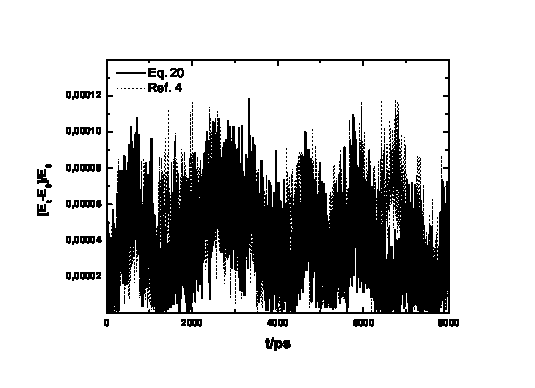
\includegraphics{millerourmd}
\captionof{figure}{Instantaneos fluctuations of energy for liquid water using Eq.~\ref{eq:trotter_splitting_NVE} (solid line) and Ref.\citenum{Miller2002} (dotted line) with $n = 1 $, $n_{ys} = 1$, $\Delta t = 1 fs$, $E_0 = -2799.87 \, kcal/mol $.}
\label{fig:miller1fs}
\end{figure}

In Table~\ref{table:nve} we compare the energy drift when using $n_{ys} = 1$ and $n_{ys} = 7$ in the rotational operator, Eq.~\ref{eq:ys_rot}. As expected, for a small time step of 1 fs, that further factorization is worthless. As the time step is increased, more accurate trajectories are achieved with $n_{ys} = 7 $. Nevertheless, the improvement is only marginal and all trajectories are stables exhibiting a small long-time energy drift. Thus, we proceed to analyze the NVT dynamics considering $n_{ys} = 1$.

\begin{table}[h]
\setlength{\tabcolsep}{7pt}
\caption{Average deviation of the conserved quantity ($DE$) from liquid water NVE simulations with $n_{ys}=1$ and $n_{ys}=7$  }
\centering % centering table
\begin{tabular}{| c  c  c |}  
\hline
&  \multicolumn{2}{c|}{ $D E$ }\\
\cline{2-3}
$\Delta t/fs$ &$n_{ys}=1$ &$n_{ys}=7$ \\
\hline % inserts single-line
 1 & 0.000055 & 0.000074\\
 2 & 0.00048 & 0.00031 \\
 3 & 0.0012 & 0.0011\\
 \hline
\end{tabular}
\label{table:nve}
\end{table}

It is not the purpose of this work to achieve an optimal factorization of the NVT schemes, but rather to show that a unique chain thermostat, while providing the ``proper'' sampling of the NVT ensemble, is capable of maintaining the average temperature at its specified value. In order to use a constant value for the smaller time step in the NHC and NHC* operators $(\Delta t/4)$, we factorized those operators analogously to the scheme given by Eq.~\ref{eq:splitting_rot}. Recalling that in the NVT dynamics the conserved quantity is the extended energy $\mathcal{H}^\prime$, in Table~\ref{table:denvt} we show the results of Eq.~\ref{eq:performance} as well as the average temperatures obtained in each case. It can be seen that both integrators, represented by the Eq.~\ref{eq:trotter_splitting_NHC} and Eq.~\ref{eq:trotter_splitting_*}, systematically achieve the specified temperature, regardless of the time step size. In addition, the energy drift is, at its worst, around $1 \%$.


\begin{table}[h]
\setlength{\tabcolsep}{7pt}
\begin{threeparttable}
\caption{Average deviation of the conserved quantity ($DE$) and average temperatures from liquid water simulation with NVT integration \tnote{a}\tnote{b}} 
\label{table:denvt}

\centering % centering table
\begin{tabular}{|c c c c c |}  
\hline
& \multicolumn{2}{c}{Eq.~$\ref{eq:trotter_splitting_NHC}$} &\multicolumn{2}{c|}{Eq.~$\ref{eq:trotter_splitting_*}$} \\
\cline{2-5}
$\Delta t/fs$ &$D E$ &$T/K$ &$D E$ &$T/K$\\
\hline % inserts single-line
 1  & 0.000043 & 298.16  & 0.000052  & 298.15 \\

 2  & 0.00013 & 298.23  & 0.00017 & 298.06  \\

 3  & 0.00089 & 298.17  & 0.0013 & 298.12  \\

 \hline
\end{tabular}
\begin{tablenotes}
\item[a] The standard deviation of the mean temperature for all cases is $\sigma = 0.037$
\item[b] The smaller time step in the NHC and NHC* operators is 0.25 fs 
\end{tablenotes}
\end{threeparttable}
\end{table}

\subsection{Partition of Energy}
\label{sec:energypartition}

Checking the consistency between the equipartition of energy and the simulated energies serves as another approach for investigating the precision of a simulation. In fact, as stated by Eastwood~\textit{et al.}~\cite{Eastwood_2010}, it has been useful to improve methodologies related to the calculation of electrostatic\cite{Levitt_1988,Guenot_1992,Arnold_1994} and dispersive\cite{Sagui_1999} interactions, as well as to detect errors in thermostats\cite{Harvey_1998,Mor_2008} and barostats\cite{Feller_1995}. The truncation error associated to the numerical schemes is a potential source of error, and is the focus of the work of Eastwood~\textit{et al.}~\cite{Eastwood_2010}, which investigates a solvated protein and a temperature difference of approximately 5.5 $K$ is observed between the protein and the solvent using a time step of 2 fs.

In this paper, we analyze the partition of energy between the translational and rotational DOF, which are related to the temperature by the equipartition theorem as follows
\begin{align}
\label{eq:tras_equipartition}
2 \langle E_{kin}^{trans} \rangle = (3N - 3) k_b T
\end{align}

\begin{align}
\label{eq:rot_equipartition}
2 \langle E_{kin}^{rot} \rangle = 3N k_b T
\end{align} 
In these equations, $N$ is the number of rigid bodies. In NVE MD simulations, conservation of total linear momentum, $ \boldsymbol{P}= cte $, results in the loss of three translational DOF : $ 3N-3 $. For a cubic box with PBC there is no rotational symmetry ~\cite{Frenkel_2013,Kuzkin_2014}, with which the total angular momentum is not conserved, giving a number of rotational DOF of $3N$.  We calculate the average energy per DOF $ \langle E_{cin} \rangle_{DOF} = \langle E_{cin} \rangle /N_{DOF}$ and then we calculate both the translational and rotational energies from equipartition as follows

\begin{equation}
\langle E_{kin}^{trans}\rangle =  \langle E_{kin} \rangle_{DOF} \, (3N-3)
\end{equation}

\begin{equation}
\langle E_{kin}^{rot} \rangle =  \langle E_{kin} \rangle_{DOF} \, (3N)
\end{equation}


In the tables below we report the translational and rotational energies using Eqs.~\ref{eq:tras_equipartition} and~\ref{eq:rot_equipartition}, together with those obtained in the NVE simulations. In this case, we simulated 903 molecules of liquid water in order to examine the behavior for a cutoff distance of $13$ {\AA}, which is a more conservative criterion as it provides better numerical stability. In Table~\ref{table:water_partition_LJ-SF} we observe that for a small time step of 0.5 fs the energies are in good correspondence, which is lost when the time step is increased. This result is confirmed also in Table~\ref{table:water_partition_13A_LJ-SF} for the cutoff distance of 13 {\AA}. This allows us to prove the influence of the truncation error on in this effect, in accordance with what Eastwood~\textit{et al.}~\cite{Eastwood_2010} point out. For significant deviations, the main implication is that Eqs.~\ref{eq:tras_equipartition} and~\ref{eq:rot_equipartition} are no longer suitable for the temperature calculation, which becomes an undefined property. In the aforementioned paper, the authors introduce an alternative approach for calculating the temperature which is based on the generalized equipartition theorem applied to the Shadow Hamiltonian, which will be investigated in future work.

%\begin{table}[h]
%\centering % centering table
%\begin{threeparttable}
%\caption{Partition of kinetic energy from an NVE simulation of 903 water molecules with $r_c = 9$ \AA~ and without shifting of LJ model\tnote{a}} %($5415 grados de libertad$)}
%\begin{tabular}{| l c  c  c  c  c  c |}  
%\toprule
%\hline
% & & & \multicolumn{2}{c}{Equipartition} & \multicolumn{2}{c|}{Simulated}\\
%  & & & \multicolumn{2}{c}{of energy} & \multicolumn{2}{c|}{partition}\\
%\cline{4-7}
%$\Delta t/fs $  &$T_{sim}/K$  &$E_{total}$ &$E_{trans}$ &$E_{rot}$ &$E_{trans}$ &$E_{rot}$ \\
%\hline % inserts single-line
% 0.5 & 305.04 & 1641.21  & 820.15  & 821.06  & 820.55 & 820.66  \\
%  1  & 304.88  & 1640.36  & 819.73  & 820.63  & 820.56 & 819.80  \\
%  2  & 304.04  & 1635.87  & 817.48  & 818.39  & 820.44 & 815.43 \\
%  3  & 302.78  & 1629.10  & 814.10  & 815.00  & 819.85 & 809.25 \\
%  \hline
%\end{tabular}
%\begin{tablenotes}
%\item[a] Energies are in $kcal/mol$.
%\end{tablenotes}
%\label{table:water_partition_2}
%\end{threeparttable}
%\end{adjustbox}
%\end{table}

\begin{table}[h]
\centering % centering table
\begin{threeparttable}
\caption{Partition of kinetic energy from NVE simulation of 903 water molecules with $r_c = 9 $ {\AA} and SF-LJ\tnote{a}} %($5415 grados de libertad$)}
%\begin{adjustbox}{width=1\textwidth}
\begin{tabular}{| l c  c  c  c  c  c |}  
\hline
 & & & \multicolumn{2}{c}{Equipartition} & \multicolumn{2}{c|}{Simulated}\\
  & & & \multicolumn{2}{c}{of energy} & \multicolumn{2}{c|}{partition}\\
\cline{4-7}
$\Delta t/fs$  &$T_{sim}/K$  &$E_{total}$ &$E_{trans}$ &$E_{rot}$ &$E_{trans}$ &$E_{rot}$ \\
\hline % inserts single-line
 0.5 & 305.20  & 1642.11  & 820.60  & 821.06  & 820.60 & 821.51  \\
  1  & 304.92  & 1640.57  & 819.83  & 820.74  & 820.63 & 819.94  \\
  2  & 304.20  & 1636.74  & 817.92  & 818.82  & 820.56 & 816.18 \\
  3  & 302.97  & 1630.07  & 814.59  & 815.48  & 820.47 & 809.60  \\
  \hline
 \end{tabular}
 \begin{tablenotes}
\item[a] Energies are in $kcal/mol$.
\end{tablenotes}
\label{table:water_partition_LJ-SF}
\end{threeparttable}
%\end{adjustbox}
\end{table}

\begin{table}[h]
\centering % centering table
\begin{threeparttable}
\caption{Partition of kinetic energy from NVE simulation of 903 water molecules with $r_c = 13$ {\AA} and SF-LJ\tnote{a}} %($5415 grados de libertad$)}
%\begin{adjustbox}{width=1\textwidth}
\begin{tabular}{ |l c  c  c  c  c  c |}  
\hline
 & & & \multicolumn{2}{c}{Equipartition} & \multicolumn{2}{c|}{Simulated}\\
  & & & \multicolumn{2}{c}{of energy} & \multicolumn{2}{c|}{partition}\\
\cline{4-7}
$\Delta t/fs$  &$T_{sim}/K$  &$E_{total}$ &$E_{trans}$ &$E_{rot}$ &$E_{trans}$ &$E_{rot}$ \\
\hline % inserts single-line
 0.5 & 307.17 & 1652.71  & 825.90  & 826.81  & 825.96 & 826.75  \\
  1 & 306.98  & 1651.68  & 825.38  & 826.30  & 826.09 & 825.59  \\
  2 & 306.04  & 1646.60  & 822.85  & 823.75 & 825.57 & 821.03 \\
  3 & 304.79 & 1639.89  & 819.49  & 820.40  & 825.63 & 814.26  \\
  \hline
 \end{tabular}
 \begin{tablenotes}
\item[a] Energies are in $kcal/mol$.
\end{tablenotes}
 \label{table:water_partition_13A_LJ-SF}
\end{threeparttable}
%\end{adjustbox}
\end{table}


\subsection{Sampling Validation}
\label{sec:samplingvalidation}
In this subsection we present the results from a simple method that serves for checking the consistency between the sampled energy distributions and the theoretical ones. The procedure, introduced and implemented by Shirts ~\cite{Shirts2013}, relies on a quantitative statistical analysis of fitting and it is possible to perform linear and nonlinear fitting or a maximum likelihood approach too. This last approach does not involve any binning of the energies, hence no discretization error is present. We report the results corresponding to that method, and since it is instructive to have a graphical insight, we also show some figures of the linear fitting.

Recall that in the NVT ensemble the probability of observing an energy E is given by
\[
P(E/\beta) = Q(\beta)^{-1}\Omega(E)\exp\left(-\beta E\right),
\]
where $ \beta $ is the Boltzmann's constant, $ \Omega(E) $ is the density of states which does not depend on $ \beta $ , and $ Q(\beta) $  is the canonical partition function, linked to the Helmholtz Free Energy $ (A) $ by $A = -\beta^{-1}\ln(Q)$. 

Taking the ratio of the probability distributions at different temperatures, the unknown density of states cancels out and we get
\begin{equation}
\label{eq:probability_ratio}
\frac{P(E/\beta_2)}{P(E/\beta_1)} = exp\left[(\beta_2 A_2 - \beta_1 A_1) - (\beta_2 - \beta_1)E\right].
\end{equation}
Taking the logarithm of Eq.~\ref{eq:probability_ratio}, we obtain
\begin{equation}
\label{eq:ln_probability_ratio}
ln\frac{P(E/\beta_2)}{P(E/\beta_1)} = \left(\beta_2 A_2 - \beta_1 A_1\right) - \left(\beta_2 - \beta_1\right)E.
\end{equation}

The Eq.~\ref{eq:ln_probability_ratio} is the basis for the statistical analysis in the ensemble validation, which determines how many standard deviations the calculated slope is from the specified one,  $ \beta_2 - \beta_1 $. Note that it is independent of the unknown free energies. For a guidance on how to choose the temperature gap the reader is referred to the aforementioned paper. Given that the potential and kinetic energies are separable, the analysis can be made separately as follows

\begin{equation}
\label{eq:probability_ratio_pot}
\frac{P_{pot}(E/\beta_2)}{P_{pot}(E/\beta_1)} = \frac{Q_{pot}(\beta_1)}{Q_{pot}(\beta_2)}  exp\left[(-\beta_2 - \beta_1)E_{pot}\right]
\end{equation}

\begin{equation}
\label{eq:probability_ratio_kin}
\frac{P_{kin}(E/\beta_2)}{P_{kin}(E/\beta_1)} = \frac{Q_{kin}(\beta_1)}{Q_{kin}(\beta_2)}  exp\left[(-\beta_2 - \beta_1)E_{kin}\right]
\end{equation}
Furthermore,  it is possible to examine the consistency between the sampled kinetic energy and the corresponding Maxwell-Boltzmann distribution, which is given by the following expression:
\begin{equation}
\label{eq:mb}
P(E_{cin}) = \frac{\beta}{\sqrt{N_{DOF}\pi}} \, exp \left[-\frac{\left(\beta E_{kin} - \frac{N_{DOF}}{2}\right)^2}{N_{DOF}} \right],
\end{equation}
where $N_{DOF}$ is the number of degrees of freedom. This last equations is a normal distribution characterized by an average of $ \langle E_{kin} \rangle = (N_{DOF}/2\beta) $ and variance $\sigma^2 = N_{DOF}/2\beta^2$, valid when equipartition of energy is satisfied.

In Fig.~\ref{fig:checkensemble} we show the result from the linear regression analysis for the potential energies sampled using Eq.~\ref{eq:trotter_splitting_NHC}. In figure legends we show the averages temperatures simulated. It can be seen that the mentioned algorithm generates a distribution consistent with the canonical ensemble, and that is also true for the kinetic energies. Likewise, in Fig.~\ref{fig:mbdistribution} we observe a good correspondence between the kinetic energy distribution at $T= 304.99 K$ and the corresponding Maxwell-Boltzmann distribution We arrive at the same conclusions for the approach given by Eq.~\ref{eq:trotter_splitting_*}.

\begin{center}
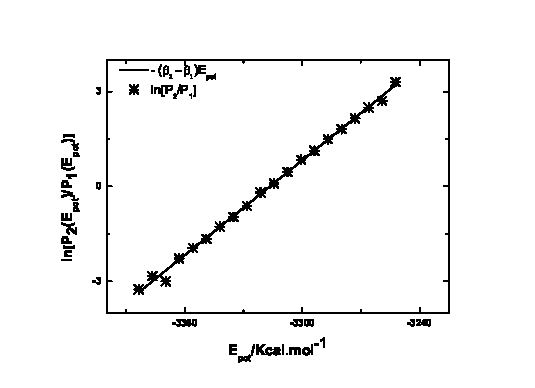
\includegraphics{checkensemble}
\captionof{figure}{Linear plot of the log ratio probabilities with the true slope (solid line) and the measured slope from the linear regression analysis (symbols). Simulation of liquid water using Eq.~\ref{eq:trotter_splitting_NHC}, $\Delta t = 1$ fs, $\bar{T}_1=296.03 K$, $\bar{T}_2 = 304.99 K$. }
\label{fig:checkensemble}
\end{center}

\begin{center}
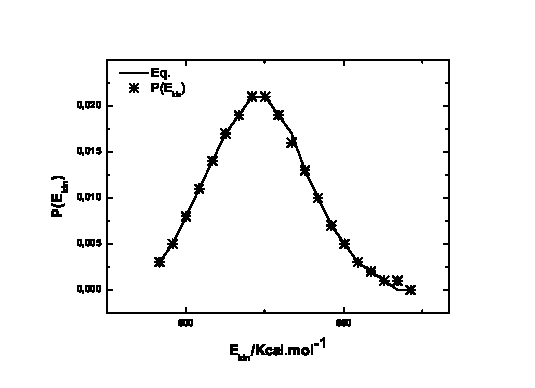
\includegraphics{maxwell-botlzamm-paper}
\captionof{figure}{Probability distribution of the kinetic energy with sampled values and those calculated with Eq.~\ref{eq:mb}. Simulation of liquid water using Eq.~\ref{eq:trotter_splitting_NHC}, $\Delta t = 1$~fs, $\bar{T} = 304.99 K$.}
\label{fig:mbdistribution}
\end{center}

Finally, in Table~\ref{table:ensemblevalidation} we present the results of the maximum likelihood approach applied for both NVT integration schemes. It can be seen that the deviations from the true slope, $\Delta T= 8.970 K $, are less than $1\sigma$. This means that effectively, the sampled values do not deviate from the correct distribution to a statistically noticeable level.

\begingroup
\squeezetable
\begin{table}
\setlength{\tabcolsep}{7pt}
\begin{threeparttable}
\caption{Ensemble Validation of NVT algorithms for liquid water using the Maximum Likelihood Approach \tnote{a} \tnote{b}}
\label{table:ensemblevalidation}
\centering % centering table
\begin{tabular}{|l c  c  c  c |}  
\hline
 & \multicolumn{4}{c|}{true $\Delta T$ = 8.970 K}\\
\cline{2-5}
  & \multicolumn{2}{c}{potential} & \multicolumn{2}{c|}{kinetic}\\
\hline
Method  &$\Delta T/K$ &$\sigma$ dev &$\Delta T/K$&$\sigma$ dev\\
\hline % inserts single-line 
 Eq.~$\ref{eq:trotter_splitting_NHC}$   & 9.022 $\pm$ 0.117 & 0.57 & 8.928 $\pm$ 0.051 & 0.63 \\
 Eq.~$\ref{eq:trotter_splitting_*}$   & 8.965 $\pm$ 0.101 & 0.05 & 8.967 $\pm$ 0.052 & 0.14\\
  \hline
\end{tabular}
\begin{tablenotes}
\item[a] The standard deviation of the mean temperature for all cases is $\sigma = 0.03$
\item[b]$\bar{T}_1 = 296.03 K $  - $\bar{T}_2 = 304.99 K$
\end{tablenotes}
\end{threeparttable}
\end{table}
\endgroup

\subsection{Pressure Calculations}

In Figure~\ref{fig:pressure} we compare the results using Eq.~\ref{eq:pressure} with those from a simulation performed with LAMMPS, which uses a numerical estimation of the constraint forces in the pressure calculation. The simulations were run in the NVE ensemble, for which neither shifting to the LJ forces nor analytical tail corrections were considered. 

%\begin{center}
%  \label{fig:pressure}
%  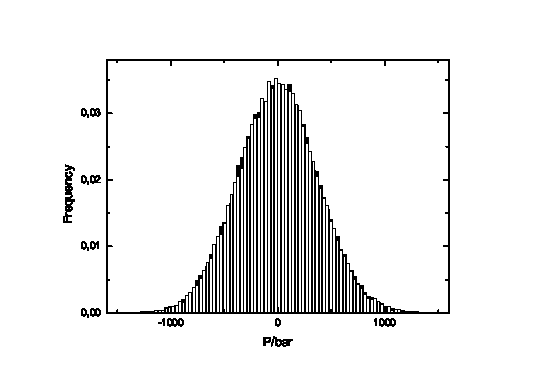
\includegraphics{pressure2}
%  \captionof{figure}{Histograms of pressure obtained in this work (filled bars) and using LAMMPS %(unfilled bars). Simulation of liquid water with NVE integration. $\Delta t : 1 fs$  }
%\end{center}

\begin{center}
\label{fig:pressure}
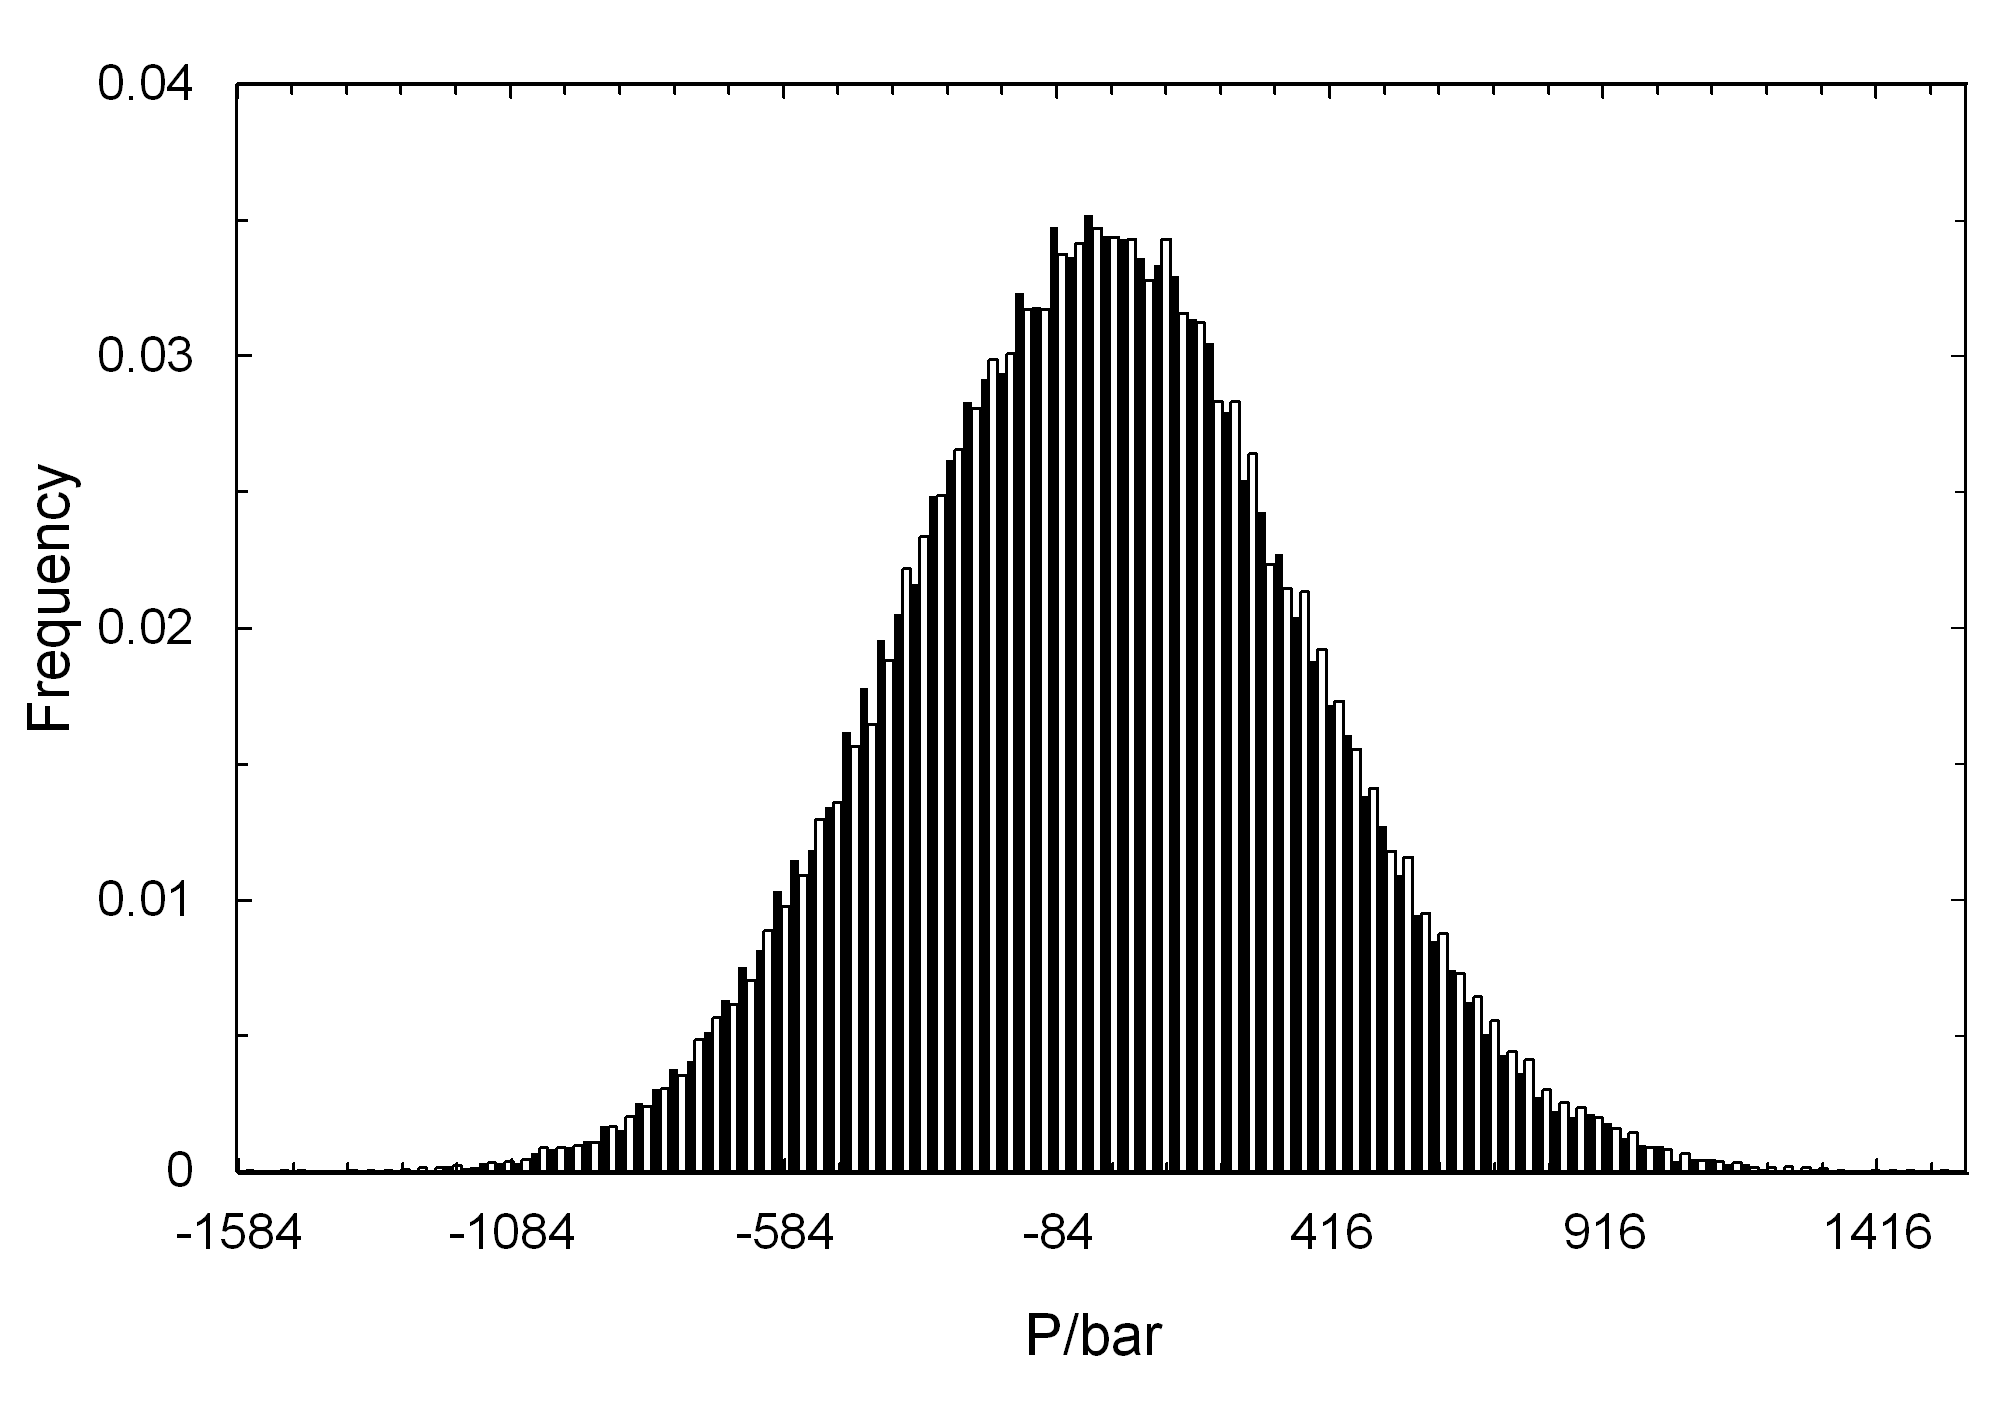
\includegraphics[width=0.5\textwidth,keepaspectratio]{FiguraAna}
\captionof{figure}{Histogram of pressure values obtained using Eq.~\ref{eq:pressure} (filled bars), along with the results from a simulation using LAMMPS (unfilled bars). The average pressures are $\bar{P} = -0.60 $ bar and $\bar{P} = 2.14 $ bar, respectively. Simulation of liquid water with NVE integration, $\Delta t = 1$ fs, $n_{ys} = 1$}
\end{center}

\subsection{To do}

Write about minimum image convention considering rigid bodies instead of atoms and about how to compute the internal virial directly using the equation below:
\[
W = \sum_{i=1}^{N-1} \sum_{k=1}^{{n_p}_i} \sum_{j=i+1}^{\infty} \sum_{l=1}^{{n_p}_j} {\vt f}_{ijkl} \cdot {\vt r}_{ij}.
\]

\appendix

\section{\label{sec:quat_from_A}Obtaining the quaternion components from a rotation matrix}

The method described here was introduced by Shepperd.\cite{Shepperd1978} As one can observe in Eq.~\ref{eq:A_from_q}, the three main diagonal components of $\mt A$ and the fact that $\lVert \vt q \lVert^2 = 1$ provide a linear system for the squares of the quaternion components whose solution is
\begin{align*}
4 q_0^2 &= 1 + tr(\mt A) \\
4 q_k^2 &= 1 + A_{k,k} - tr(\mt A)
\end{align*}
where $k = 1,2,3$ and $tr(\mt A)$ is the trace of matrix $\mt A$. Since both $\vt q$ and $- \vt q$ correspond to the same rotation matrix, the sign the largest component\cite{Shepperd1978} can be made positive and the others can be obtained from the off-diagonal entries of $\mt A$, which give
\begin{align*}
4 q_0 q_1 &= A_{2,3} - A_{3,2} \\
4 q_0 q_2 &= A_{3,1} - A_{1,3} \\
4 q_0 q_3 &= A_{1,2} - A_{2,1} \\
4 q_k q_l &= A_{k,l} + A_{l,k} \\
\end{align*}
where $k,l = 1,2,3$ with $k \neq l$.

\section{\label{sec:auxiliary_math}Algebraic relations involving unit quaternions}

Let us analyze the matrix $\mt B$ defined as in Eq.~\ref{eq:def_B_and_C}. Note that $\tr{\mt B}\vt q = \vt 0$, where $\vt 0$ is a null vector.\cite{Haug1989, Shuster1993, Dichmann1999} This means that all columns of $\mt B$ are orthogonal to $\vt q$. As these columns have unit norm and are also orthogonal to each other, they form an orthonormal basis for the hyperplane orthogonal to $\mt q$, which is a subspace of $\mathbb{R}^4$. Therefore, the general operation $\vt y = \mt B \vt x$ transforms a vector $\vt x \in \mathbb{R}^3$ into a quaternion $\vt y \in \mathbb{R}^4$, but restricted to the mentioned hyperplane. Other two identities that hold for $\mt B$ are\citep{Haug1989}
\begin{align*}
\tr{\mt B}\mt B &= \lVert \vt q \lVert ^2{\mt 1}_3 \text{ and} \\
\mt B\tr{\mt B} &= \lVert \vt q \lVert ^2{\mt 1}_4 - {\vt q}\tr{\vt q}.
\end{align*}

If $\lVert \vt q \lVert^2 = 1$, then the operation $\vt y = \mt B \vt x$ can always be reverted by $\tr{\mt B}$. This is not true for a general operation in the opposite direction, $\vt x = \tr{\mt B} \vt y$. Besides unit norm, it is necessary that $\tr{\vt q}\vt y = 0$ (i.e. orthogonality of $\vt y$ and $\vt q$) for the operation to be reversible by $\mt B$. In fact, the composite transformation $\mt B\tr{\mt B}$ corresponds to a projection into the hyperplane orthogonal to $\vt q$.\cite{Dichmann1999}

All the conclusions drawn thus far for matrix $\mt B$ are equally valid for matrix $\mt C$.

As the columns of $\mt B$ are permutations of the Euler parameters, one can write $\mt B = [\begin{array}{ccc}{\mt B}_1{\vt q} & {\mt B}_2{\vt q} & {\mt B}_3{\vt q}\end{array}]$, where $\mt B_1$, $\mt B_2$, and $\mt B_3$ are permutation matrices given by
\[
{\mt B}_1 = \left[ \begin{array}{rrrr}
 0 & -1 &  0 &  0 \\
 1 &  0 &  0 &  0 \\
 0 &  0 &  0 &  1 \\
 0 &  0 & -1 &  0 \\
\end{array} \right], \;
{\mt B}_2 = \left[ \begin{array}{rrrr}
 0 &  0 & -1 &  0 \\
 0 &  0 &  0 & -1 \\
 1 &  0 &  0 &  0 \\
 0 &  1 &  0 &  0 \\
\end{array} \right],
\]\[
\text{and }{\mt B}_3 = \left[ \begin{array}{rrrr}
 0 &  0 &  0 & -1 \\
 0 &  0 &  1 &  0 \\
 0 & -1 &  0 &  0 \\
 1 &  0 &  0 &  0 \\
\end{array} \right].
\]

All these permutation matrices are skew-symmetric (i.e. $\tr{\mt B_k} = -\mt B_k$) and also satisfy the relations\cite{Dichmann1999}
\begin{equation}
\label{eq:BB_products}
\begin{aligned}
\tr{\mt B_1}{\mt B_1} &= \tr{\mt B_2}{\mt B_2} = \tr{\mt B_3}{\mt B_3} = \mt 1_3 \\
\tr{\mt B_1}{\mt B_2} &= -\tr{\mt B_2}{\mt B_1} = -\tr{\mt B_3} \\
\tr{\mt B_2}{\mt B_3} &= -\tr{\mt B_3}{\mt B_2} = -\tr{\mt B_1} \\
\tr{\mt B_3}{\mt B_1} &= -\tr{\mt B_1}{\mt B_3} = -\tr{\mt B_2}
\end{aligned}
\end{equation}

The product of $\mt B$ with an arbitrary vector $\vt x$ results in
\begin{equation}
\label{eq:product_B_vector}
\mt B \vt x = \left[ \begin{array}{ccc} \mt B_1 \vt q & \mt B_2 \vt q & \mt B_3 \vt q \end{array}\right] \left[ \begin{array}{c} x_1 \\ x_2 \\ x_3 \end{array} \right] = \sum_{k=1}^3 x_k {\mt B}_k \vt q.
\end{equation}

Similarly, the product of $\tr{\mt B}$ with an arbitrary quaternion $\vt y$ results in
\begin{equation}
\label{eq:vector_entries}
\tr{\mt B}\vt y =
\left[\begin{array}{c}
\tr{\vt q}\tr{\mt B}_1 \\
\tr{\vt q}\tr{\mt B}_2 \\
\tr{\vt q}\tr{\mt B}_3 \\
\end{array}\right]\vt y = 
\left[\begin{array}{c}
\tr{\vt q}\tr{\mt B}_1\vt y \\
\tr{\vt q}\tr{\mt B}_2\vt y \\
\tr{\vt q}\tr{\mt B}_3\vt y \\
\end{array}\right] = 
\left[\begin{array}{c}
\tr{\vt y}{\mt B}_1\vt q \\
\tr{\vt y}{\mt B}_2\vt q \\
\tr{\vt y}{\mt B}_3\vt q \\
\end{array}\right].
\end{equation}

Let us now consider the product $\tr{\mt B}\dot{\mt B}$, where $\dot{\mt B}$ is the time derivative of $\mt B$. Because the permutation matrices are constant, we can express $\dot{\mt B} = [\begin{array}{ccc}{\mt B}_1\dot{\vt q} & {\mt B}_2\dot{\vt q} & {\mt B}_3\dot{\vt q}\end{array}]$. By carrying out the multiplication and applying the relations of Eq.~\ref{eq:BB_products}, we observe that
\[
\tr{\mt B}\dot{\mt B} = \left[
\begin{array}{ccc}
0 & -\tr{\vt q} \tr{\mt B_3}\dot{\vt q} & \tr{\vt q} \tr{\mt B_2}\dot{\vt q} \\
\tr{\vt q} \tr{\mt B_3}\dot{\vt q} & 0 & -\tr{\vt q} \tr{\mt B_1}\dot{\vt q} \\
-\tr{\vt q} \tr{\mt B_2}\dot{\vt q} & \tr{\vt q} \tr{\mt B_1}\dot{\vt q}  & 0
\end{array}
\right],
\]
where the diagonal entries are zero as a consequence of the orthogonality between $\vt q$ and $\dot{\vt q}$. By contrasting this result with Eq.~\ref{eq:operator_S}, we draw the conclusion that
\begin{equation}
\label{eq:relation_B_qdot}
\tr{\mt B}\dot{\mt B} = {\mt S}\left( \tr{\mt B}\dot{\vt q} \right).
\end{equation}

Matrix $\mt C$ and its time-derivative $\dot{\mt C}$ can also be expressed as $[\begin{array}{ccc}{\mt C}_1{\vt q} & {\mt C}_2{\vt q} & {\mt C}_3{\vt q}\end{array}]$ and $[\begin{array}{ccc}{\mt C}_1\dot{\vt q} & {\mt C}_2\dot{\vt q} & {\mt C}_3\dot{\vt q}\end{array}]$, respectively, where $\mt C_1$, $\mt C_2$, and $\mt C_3$ are
\[
{\mt C}_1 = \left[ \begin{array}{rrrr}
 0 & -1 &  0 &  0 \\
 1 &  0 &  0 &  0 \\
 0 &  0 &  0 & -1 \\
 0 &  0 &  1 &  0 \\
\end{array} \right], \;
{\mt C}_2 = \left[ \begin{array}{rrrr}
 0 &  0 & -1 &  0 \\
 0 &  0 &  0 &  1 \\
 1 &  0 &  0 &  0 \\
 0 & -1 &  0 &  0 \\
\end{array} \right],
\]\[
\text{and }{\mt C}_3 = \left[ \begin{array}{rrrr}
 0 &  0 &  0 & -1 \\
 0 &  0 & -1 &  0 \\
 0 &  1 &  0 &  0 \\
 1 &  0 &  0 &  0 \\
\end{array} \right].
\]

A special connection between the permutation matrices for $\mt B$ and $\mt C$ is the fact that $\tr{\mt B_i}{\mt C_j}$ is symmetric for any combination of $i$ and $j$. Thus, each entry of $\tr{\mt B}\dot{\mt C}$ is
\begin{align*}
\{\tr{\mt B}\dot{\mt C}\}_{ij} &= \tr{\vt q}\tr{\mt B}_i{\mt C}_j\dot{\vt q} = \tr{\vt q}\tr{\mt C}_j{\mt B}_i\dot{\vt q} = \{\tr{\mt C}\dot{\mt B}\}_{ji} = \\
&= \{\tr{\dot{\mt B}}\mt C\}_{ij}.
\end{align*}

This means that $\tr{\mt B}\dot{\mt C} = \tr{\dot{\mt B}}{\mt C}$. Proceeding further, we observe that
\begin{align*}
\mt A \tr{\dot{\mt A}} &= \tr{\mt B}\mt C \tr{(\tr{{\mt B}}\dot{\mt C} + \tr{\dot{\mt B}}{\mt C})} = \tr{\mt B}\mt C \tr{(2 \tr{\dot{\mt B}}{\mt C})} = \\
&= 2 \tr{\mt B}\dot{\mt B},
\end{align*}
where we have applied the relations $\mt C \tr{\mt C} = \mt 1_4 - \vt q\tr{\vt q}$ and $\tr{\vt B}\vt q = \vt 0$. Finally, resorting to Eqs.~\ref{eq:relation_A_omega} and \ref{eq:relation_B_qdot}, the result above converts to
\begin{equation}
\vt \omega = 2\tr{\mt B}\dot{\vt q}.
\end{equation}

\begin{equation}
\label{eq:operator_S}
\mt S(\vt x) = \left[ \begin{array}{ccc}
0   & -x_3 &  x_2 \\
x_3 &  0   & -x_1 \\
-x_2 &  x_1 &  0
\end{array}\right].
\end{equation}

The operator  $\mt S(\cdot)$ is able to represent the cross-product of two vectors $\vt x$ and $\vt y$ as a matrix-vector product, since $\vt x \times \vt y = \mt S(\vt x)\vt y$. This property is explored in the Appendix.

Demonstration of Euler equation:

\begin{align*}
\diff{(\tr{\mt B}\vt \pi)}{t} &= \tr{\dot{\mt B}}\vt \pi + \tr{\mt B}\dot{\vt \pi} = \\
&=\tr{\dot{\mt B}}{\mt B}\tr{\mt B}{\vt \pi}  + \dfrac{1}{2} \tr{\mt B}\mt \Omega \vt \omega + 2 \tr{\mt B}\mt C \vt \tau = \\
&= -\frac{1}{2}{\mt S}(\vt \omega)\tr{\mt B}{\vt \pi} + \dfrac{1}{2} {\mt S}(\tr{\mt B}\mt \pi) \vt \omega + 2 \mt A \vt \tau = \\
&= - \vt \omega \times (\tr{\mt B}{\vt \pi}) + 2 {\vt \tau}^\prime
\end{align*}

As $\tr{\mt B}\vt \pi = 2 \mt I \vt \omega$, the result above becomes
\[
\mt I \dot{\vt \omega} + \vt \omega \times (\mt I \vt \omega) = {\vt \tau}^\prime
\]

\section{\label{sec:Diff_Rules}Differentiation rules with vectors}

Along the paper, the differentiation of scalar functions with respect to vectors are done directly using the following rules:
\[
\diff{(\tr{\vt x}\vt a)}{\vt x} = \diff{(\tr{\vt a}\vt x)}{\vt x} = \vt a
\]
and
\[
\diff{(\tr{\vt x}\mt A \vt x)}{\vt x} = 2 \mt A \vt x,
\]
where $\vt a$ is vector and $\mt A$ is a matrix, both independent of $\vt x$.

\section{\label{sec:Diff_PotEng}Potential energy differentiation}

Care must be taken when differentiating the potential energy $U$ with respect to $\vt q$ because the Euler parameters are not all independent. Schay demonstrated in Ref.~\cite{Schay1995} that, when differentiating a scalar function $f$ with respect to a vector variable $\vt x$, subject to a constraint $g(\vt x) = 0$, the derivative of $f$ with respect to $\vt x$ is given by
\[
\diff{f}{\vt x} = (\vt 1 - \vt n \tr{\vt n})\left( \diff{f}{\vt x} \right)^\ast,
\]
where $\vt n$ is the unit vector proportional to $(\partial g/\partial \vt x)^\ast$, with the asterisk denoting a differentiation performed without considering the interdependence of the entries of $\vt x$. We note that transpositions are necessary when comparing the equation above, based on the gradient convention, with that in Ref.~\cite{Schay1995}, where the Jacobian convention is used. In the  case of Euler parameters,
\[
g(\vt q) = \tr{\vt q}\vt q - 1 \; \rightarrow \; \left(\diff{g}{\vt q}\right)^\ast = 2 \vt q.
\]

Hence, the unit four-dimensional vector proportional to $(\partial g/\partial \vt x)^\ast$ is exactly $\vt q$, which means that the constrained derivative of $U$ is given by
\begin{equation}
\label{eq:diff_projection}
\diff{U}{\vt q} = (\mt 1_4 - {\vt q}\tr{\vt q})\left( \diff{U}{\vt q} \right)^\ast.
\end{equation}

Therefore, the constrained derivative is the projection of the unconstrained one in the hyperplane orthogonal to $\vt q$. Recently, Nielsen and Krenk\cite{Nielsen2012} employed a Lagrange multiplier approach to demonstrate the need of carrying out such projection. Schay\cite{Schay1995, Schay1998} discussed on the equivalence of the two approaches.

By applying the chain rule, we have
\[
\left( \diff{U}{\vt q} \right)^\ast = \sum_{j=1}^{n_p} \left( \diff{\vt R_j}{\vt q} \right)^\ast \diff{U}{\vt R_j} = - \sum_{j=1}^{n_p} \left( \diff{\vt R_j}{\vt q} \right)^\ast {\vt F_j},
\]
where $\vt F_j = -\partial U/\partial \vt R_j$ is, by definition, the force applied on particle $j$. As $\vt R_j = \vt r + \tr{\mt A}\vt d_j$,
\[
\left( \diff{\vt R_j}{\vt q} \right)^\ast = \left( \diff{(\tr{\mt A}\vt d_j)}{\vt q} \right)^\ast.
\]

For simplicity, we will drop the index $j$ for the next few lines. Remember that $\tr{\mt A}\vt d = \tr{\mt C} \mt B\vt d$ and, according to Eq.~\ref{eq:product_B_vector},
\[
\mt B \vt d = \sum_{k=1}^3 d_k \mt B_k \vt q = \left( \sum_{k=1}^3 d_k \mt B_k \right) \vt q.
\]

An identity equivalent to Eq.~\ref{eq:vector_entries} holds for the product of $\tr{\mt C}$ with an arbitrary quaternion, so that we can write
\[
\tr{\mt A}{\vt d} =
\left[\begin{array}{c}
\tr{\vt q}\tr{\mt C}_1 \mt B \vt d \\
\tr{\vt q}\tr{\mt C}_2 \mt B \vt d \\
\tr{\vt q}\tr{\mt C}_3 \mt B \vt d \\
\end{array}\right] = 
\left[\begin{array}{c}
\tr{\vt q} \tr{\mt C}_1 \left( \sum_{k=1}^3 d_k \mt B_k \right) \vt q \\
\tr{\vt q} \tr{\mt C}_2 \left( \sum_{k=1}^3 d_k \mt B_k \right) \vt q \\
\tr{\vt q} \tr{\mt C}_3 \left( \sum_{k=1}^3 d_k \mt B_k \right) \vt q \\
\end{array}\right].
\]

As mentioned in Appendix \ref{sec:auxiliary_math}, $\tr{\mt C}_i \mt B_j = \tr{\mt B}_j \mt C_i$ for any pair $ij$, so that all the constant matrices above between $\tr{\vt q}$ and $\vt q$ are constant and symmetric, which facilitates differentiation. After carrying it out and replacing back $(\sum_{k=1}^3 d_k \mt B_k) \vt q$ by $\mt B \vt d$, we have
\[
\left( \diff{\vt R}{\vt q} \right)^\ast = 2 \left[\begin{array}{ccc}
\tr{\mt C}_1 \mt B \vt d & \tr{\mt C}_2 \mt B \vt d & \tr{\mt C}_3 \mt B \vt d
\end{array}\right]
\]

Considering that we deal exclusively with unit quaternions $\vt q$, so that $\mt C \tr{\mt C} = \mt 1_4 - \vt q \tr{\vt q}$ can be substituted in Eq.~\ref{eq:diff_projection}, it is useful to evaluate the product
\[
\tr{\mt C} \left( \diff{\vt R}{\vt q} \right)^\ast = 2 \left[\begin{array}{c}
\tr{\vt q}\tr{\mt C_1} \\
\tr{\vt q}\tr{\mt C_2} \\
\tr{\vt q}\tr{\mt C_3}
\end{array}\right] \left[\begin{array}{ccc}
\tr{\mt C}_1 \mt B \vt d & \tr{\mt C}_2 \mt B \vt d & \tr{\mt C}_3 \mt B \vt d
\end{array}\right]
\]

The permutation matrices $\mt C_1$, $\mt C_2$, and $\mt C_3$ have the following properties:
\begin{equation}
\begin{aligned}
\tr{\mt C_1}\tr{\mt C_1} &= \tr{\mt C_2}\tr{\mt C_2} = \tr{\mt C_3}\tr{\mt C_3} = -\mt 1_4 \\
\tr{\mt C_1}\tr{\mt C_2} &= -\tr{\mt C_2}\tr{\mt C_1} = -\tr{\mt C_3} \\
\tr{\mt C_2}\tr{\mt C_3} &= -\tr{\mt C_3}\tr{\mt C_2} = -\tr{\mt C_1} \\
\tr{\mt C_3}\tr{\mt C_1} &= -\tr{\mt C_1}\tr{\mt C_3} = -\tr{\mt C_2}
\end{aligned}
\end{equation}

Along with the fact that $\mt B\vt d$ and $\vt q$ are necessarily orthogonal to each other, the properties above lead to
\begin{align*}
\tr{\mt C} \left( \diff{\vt R}{\vt q} \right)^\ast &= 2 \left[\begin{array}{ccc}
0 & -\tr{\vt q}\tr{\mt C}_3 \mt B \vt d & \tr{\vt q}\tr{\mt C}_2 \mt B \vt d \\
\tr{\vt q}\tr{\mt C}_3 \mt B \vt d & 0 & -\tr{\vt q}\tr{\mt C}_1 \mt B \vt d \\
-\tr{\vt q}\tr{\mt C}_2 \mt B \vt d & \tr{\vt q}\tr{\mt C}_1 \mt B \vt d & 0
\end{array}\right] \\
&= 2 \mt S(\tr{\mt C} \mt B \vt d) = 2 \mt S(\tr{\mt A}\vt d) = 2 \mt S(\vt \delta),
\end{align*}
where $\vt \delta$ is equivalent to $\vt d$, but expressed in the space-fixed frame of reference. Finally, we obtain
\[
\diff{U}{\vt q} = - 2 \mt C \sum_{j=1}^{n_p} \mt S(\vt \delta_j) {\vt F_j}  = - 2 \mt C \sum_{j=1}^{n_p} \vt \delta_j \times {\vt F_j}.
\]


\bibliography{rigid_bodies}

\end{document}
